% ***************************** MAIN FILE **********************************

\documentclass[12pt]{scrreprt}           % Art des zu erstellenden Dokuments
% bei zweiseitigem Druck twoside-Option oder book-Klasse verwenden

% ****************************** PREAMBLE **********************************
% **************************** PACKAGE SETUP *******************************
\usepackage[ngerman]{babel}          % Lokalisierung von Typographie, Silbentrennung, etc.

\usepackage{ucs}                     % Erweiterte Unterstützung von UTF-8-Kodierung
\usepackage[utf8x]{inputenc}         % Unterstützung von UTF-8 in Eingabe-Dateien
\usepackage[T1]{fontenc}             % Zeichensatzkodierung von LaTeX (Cork-Kodierung)
\usepackage{helvet,courier,mathptmx} % Verwendete Schriftarten

\usepackage[headsepline, plainheadsepline, plainfootsepline] {scrlayer-scrpage}

\usepackage{amsmath}                 % Mathematische Infrastruktur für LaTeX der AMS
\usepackage{amsfonts}                % Mathematische Schriftarten
\usepackage{amssymb}                 % Mathematische Symbole
\usepackage{amsthm}                  % Erweiterung der Theorem-Umgebungen
\usepackage[]{units}				 % für \unit-Befehl
%\usepackage[amssymb]{siunits}		 % für SI-Einheiten (amssymb definiert den Befehl \square des amssymb Packages um. Ist dies nicht gewünscht kann die Option squaren verwendet werden. Dann muss für die SI-Einheiten \squaren anstatt \square verwendet werden.)

%\usepackage{fancyhdr}               % Erweiterte Konfiguration von Kopf/Fußzeile
\usepackage{hyperref}                % Querverweise, Hyperlink, pdf-Konfiguration, etc.

\usepackage{float}                   % Selbstdefinierte Floating-Umbgebungen
\usepackage{tabularx}                % Tabellen mit einstellbarer Spaltenbreite
\usepackage[labelfont=bf]{caption}   % Anpassen der Abbildungs- und Tabellenbeschriftungen

\usepackage{algpseudocode}           % Algorithmen als Pseudocode (basiert auf algorithmicx)
\usepackage{listings}                % Quellcode-Satz (z.B. mit Syntax-Hervorhebung)
\lstset { %
    language=Python,
    backgroundcolor=\color{black!5}, % set backgroundcolor
    basicstyle=\footnotesize,        % basic font setting
}

\usepackage[pdftex,
%draft							     %Figures werden nur als Platzhalter eingeblendet
]{graphicx}						     % Erweiterte Unterstützung von Graphiken
\usepackage{textpos}                 % Beliebig platzierte Textboxen
\usepackage{xcolor}                  % TeX-Engine-unabhängige Definition von Farben
\usepackage{acronym}


\usepackage{pdfpages}

\usepackage[numbers]{natbib}         % Weiter Optionen für die Bibliographie
\usepackage{todonotes}
\usepackage{tabulary}
\usepackage{IEEEtrantools}
\usepackage{multicol}
\usepackage{graphicx}
\usepackage{enumitem}
\usepackage{tabularx}


% ****************************** TOP MATTER ***********************************
\newcommand{\studenteins}{Erkan Garan}           % Name
\newcommand{\matrNumbereins}{70467533}              % Matrikelnummer
\newcommand{\studycourse}{Informatik}           % Studiengang

\newcommand{\supervisor}{Prof. Dr. Claus Fühner, Stefan Jung} % Betreuer
\newcommand{\institution}{Ostfalia Hochschule} % Hochschule
\newcommand{\subinstitution}{Hochschule Braunschweig/Wolfenbüttel}
\newcommand{\faculty}{Informatik}               % Fachbereich
\newcommand{\toponym}{Wolfenbüttel}                 % Ort

\renewcommand{\subject}{Bachelorarbeit}  % Art/Thema der Arbeit
\newcommand{\titel}{{Entwurf eines Modells für ein unterstützendes KI-System zur Bewertung von Anwendungsregeln}} % Titel der Arbeit
\newcommand{\subtitel}{} % Untertitel
\newcommand{\graduation}{Bachelor of Science} % Angestrebter Titel (nur bei Abschlussarbeiten, sonst leer lassen/auskommentieren)

\newcommand{\keywords}{{}} % Stichworte (durch Komma getrennt)


% **************************** HYPERREF SETUP *******************************
\definecolor{linkcolor}{rgb}{1,0.5,0}
\hypersetup
{
bookmarks=true,                        % Lesezeichen im PDF erzeugen
bookmarksopen=true,                    % Lesezeichen im PDF sofort anzeigen
backref=true,                          % Rückverweise im Literaturverzeichnis
colorlinks=true,                       % Farbige Verweise
%hidelinks = true,                      % Verweise verbergen (entfernt Farbe und Rahmen)
pdfstartview={FitH},                   % Ansicht des PDFs beim öffnen
pdftitle={\titel},                     % Title des PDFs
pdfauthor={\author , \supervisor},     % Autor des PDFs
pdfsubject={\subject},                 % Thema des PDFs
%pdfcreator={Creator},                 % Erzeuger des Dokuments (Anwendungsprogramm)
%pdfproducer={Producer},               % Ersteller des PDFs (Programm/Bibliothek/Skript)
pdfkeywords={\keywords},               % Stichwörter zum PDF
linkcolor=linkcolor,                   % Farbe von Querverweisen
citecolor=green,                       % Farbe von Zitaten
filecolor=magenta,                     % Farbe von Verweisen auf Dateien
urlcolor=cyan                          % Farbe von URLs
}
% Weitere Optionen: http://www.tug.org/applications/hyperref/manual.html

% **************************** LISTINGS SETUP *******************************
\definecolor{keywords}{rgb}{0.5 0 0.3}
\definecolor{comments}{rgb}{0.25,0.5,0.37}
\lstset{ %
  backgroundcolor=\color{white},   % Hintergrundfarbe
  basicstyle=\linespread{0.94}\footnotesize\ttfamily, % Schrifteinstellungen für Quellcode
  breakatwhitespace=false,         % Automatische Zeilenumbrüche nur bei Leer- oder Tabulatorzeichen (Leerraum/whitespaces)
  breaklines=true,                 % Automatische Zeilenumbrüche
  captionpos=b,                    % Beschriftung unten
  commentstyle=\color{comments},   % Schrifteinstellungen für Kommentare
%  deletekeywords={...},            % Bestimmte Schlüsselwörter entfernen
  escapeinside={\%*}{*)},          % Defintion von Escape-Sequenzen
  extendedchars=true,              % Nicht ASCII-Zeichen erlauben
  frame=single,                    % Rahmen um den Quellcode
  keepspaces=true,                 % Einrückungen im Quellcode behalten
  keywordstyle=\bfseries\color{keywords},% Schrifteinstellungen für Schlüsselwörter
  language=java,                   % Programmiersprache des Quellcodes
%  morekeywords={*,...},            % Zusätzliche Schlüsselwörter
  numbers=left,                    % Zeilennummerierung
  numbersep=5pt,                   % Abstand zwischen Zeilennummerierung und Quellcode
  numberstyle=\tiny\color{gray}, % Schrifteinstellungen für Zeilennummern
  rulecolor=\color{black},         % if not set, the frame-color may be changed on line-breaks within not-black text (e.g. comments (green here))
  showspaces=false,                % Leerraum-Zeichen anzeigen
  showstringspaces=false,          % Leerzeichen in Zeichenketten anzeigen
  showtabs=false,                  % Tabulatorzeichen in Zeichenketten anzeigen
  stepnumber=1,                    % Schrittweite bei Zeilennummern
  stringstyle=\color{blue},        % Schrifteinstellungen für Zeichenketten
  tabsize=4,                       % Tabulatorbreite (Anzahl Leerzeichen)
  numberbychapter=false            % Nummeriere Quellcode fortlaufend je Kapitel
}
\renewcommand{\lstlistlistingname}{Quellcodeverzeichnis}
\renewcommand{\lstlistingname}{Quellcode}

\AtBeginDocument{\numberwithin{lstlisting}{section}} % Nummeriere Quellcode fortlaufend je Abschnitt

% ************************** HEADER/FOOTER SETUP ****************************
\pagestyle{scrheadings}

\clearscrheadings				% löscht voreingestellte Stile
\clearscrplain					% löscht voreingestellte Stile

\lohead[\headmark]{\headmark}
\rohead[\pagemark]{\pagemark}

\automark{chapter}

% **************************** GRAPHICX SETUP *********************************
\DeclareGraphicsExtensions{.pdf,.png,.jpg} % bekannte Graphik-Dateiformate (müssen nicht mehr im Dateinamen angegeben werden, also statt "beispiel.png" nur noch "beispiel")
\graphicspath{{./figure/}}   % path to graphics folder, usage {PATH},{ANOTHERPATH}...

% ************************** BIBLIOGRAPHY SETUP ********************************
\bibliographystyle{IEEEtranN}    % Literaturverzeichnis nach IEEE
%\AtBeginDocument{\nocite{*}} % Diese Zeile vor der Abgabe der Arbeit entfernen!

% ****************************** MATH SETUP ************************************
\everymath{\displaystyle}    % Erzwinge \displaystyle für Mathematischen-Modus


% ************************* THEOREMS AND PROOF *********************************
\newtheoremstyle{thesis}     % Name des neuen Theorem-Stils
{3pt}                        % Abstand oberhalb des Theorems
{3pt}                        % Abstand unterhalb des Theorems
{\itshape}                   % Schrifteinstellungen innerhalb des Theorems
{}                           % Einrückung der Theorem-Überschrift
{\bfseries}                  % Schrifteinstellungen für die Überschrift des Theorems
{}                           % Satzzeichen zwischen Überschrift und Theorem-Rumpf
{\newline}                   % Abstand hinter der Überschrift
{}                           % Spezifikation der Überschrift
  
\theoremstyle{thesis}        % Verwende neuen Theorem-Stil

\newtheorem{theorem}{Satz}[section] % neue Theorem-Umgebung: theorem (Satz)
\providecommand*{\theoremautorefname}{Satz} % autoref-Name für theorem

\newtheorem{definition}{Definition}[section] % neue Theorem-Umgebung: definition (Definition)
\providecommand*{\definitionautorefname}{Definition} % autoref-Name für definition

\renewcommand{\qedsymbol}{$\blacksquare$} % Schwarzes Quardrat als Symbol für: q. e. d.
\renewenvironment{proof}[1][\proofname]{{\bfseries #1:}~}{\qed} % "Beweise:" in Fettdruck

% *************************** PSEUDOCODE SETUP ********************************
\floatstyle{boxed}                        % Rahmen für pseudocode-Umgebung
\newfloat{pseudocode}{htbp}{lop}[section] % Definieren pseudocode-Umgebung
\floatname{pseudocode}{Pseudocode}        % Beschrifte pseudocode-Umgebung mit "Pseudocode"

\newcommand{\listofpseudocodename}{Pseudocodeverzeichnis}
\newcommand{\listofpseudocode}{\listof{pseudocode}{\listofpseudocodename}}
\providecommand*{\pseudocodeautorefname}{Pseudocode}

% ******************************* PAGE SETUP **********************************
\textheight23cm
\textwidth14cm
\voffset0cm
\topskip0cm
\topmargin-1.2cm
\headheight1.0cm
\headsep1.5cm
\oddsidemargin1.0cm
\evensidemargin1.0cm
\renewcommand{\baselinestretch}{1.4} 

% Hurenkinder und Schusterjungen verhindern
\clubpenalty = 10000
\widowpenalty = 10000
\displaywidowpenalty = 10000

% Verbesserung der Textsetzung
\tolerance = 1000
\emergencystretch = 20pt

% ******************************** MACROS *************************************
\newcommand{\RR}{\mathbf{R}}
\newcommand{\NN}{\mathbf{N}}
\newcommand{\QQ}{\mathbf{Q}}
\newcommand{\ZZ}{\mathbf{Z}}
\newcommand{\CC}{\mathbf{C}}
\newcommand{\erstelltvon}[1]{\marginpar{\fbox{#1}}}


\setcounter{tocdepth}{1} % Entfernt subsections aus dem Inhaltsverzeichnis

%%%%%%%%%%%%%%%%%%%%%%%%%%%%%%%%%%%%%%%%%%%%%%%%%%%%%%%%%%%%%%%%%%%%%%%%%%%%%%%
% ************************** BEGINN OF DOCUMENT *******************************
%%%%%%%%%%%%%%%%%%%%%%%%%%%%%%%%%%%%%%%%%%%%%%%%%%%%%%%%%%%%%%%%%%%%%%%%%%%%%%%
\begin{document}
\bstctlcite{IEEEexample:BSTcontrol} 
\pagestyle{plain}

% 
%% *** Titelseite ***
%
\begin{titlepage}
	\vspace*{-3.0cm}
	%Logo international
	%\hspace*{ 9.30cm}
\includegraphics[scale=0.93]{../ostfalia/LSVorlagejpg_klein_int.jpg}\\
	%Logo deutsch
	%\hspace*{10.20cm}
\includegraphics[scale=0.60]{../ostfalia/Ostfalia_LS_RGB_klein.jpg}\\
	\hspace*{ 6.90cm}
\includegraphics[scale=0.93]{../ostfalia/Ostfalia_LS_RGB_klein.jpg}\\
	%Logo ohne Schrift
	%\hspace*{15.00cm}
\includegraphics[scale=0.60]{../ostfalia/Ostfalia_L_RGB_klein.jpg}\\
	%\hspace*{14.30cm}
\includegraphics[scale=0.93]{../ostfalia/Ostfalia_L_RGB_klein.jpg}\\
	\hspace*{-1.00cm}
\includegraphics[scale=1.20]{../ostfalia/Reiter_Wolfen_RGB_174mm.jpg}\\
	
	\hspace*{-0.5cm}{\Large\textsf{Fakultät \faculty}}\\
	
	\hrulefill\\
	
	%-------------------------------------------------------------------------------
	\noindent{\Large\textsf{\studenteins, \matrNumbereins\\}}
	\ifdefined\studentzwei%
	\if\studentzwei\empty
	\else
	{\Large\textsf{\studentzwei, \matrNumberzwei\\}}
	\fi
	
	
	\vspace{2em}
	\textbf{
	\textsf{\huge\titel \\[0.3ex]}}
	\textsf{\hspace*{0.5cm}\large \subtitel \\[0.05cm]}
	
	\vspace{2em}
	\begin{center}
	\ifdefined\graduation%
	\if\graduation\empty%
	\else%
	\textsf{Abschlussarbeit zur Erlangung des akademischen Grades}\\[0.5cm]
	\textsf{\graduation} \textsf{im Studiengang Informatik}\\[0.5cm]
	\textsf{an der \institution}\\[0.5cm]
	\textsf{\subinstitution}
	\fi
	\end{center}
	
	\vspace*{\fill}

 	\enlargethispage{1\baselineskip}
	\hrulefill\\
	\begin{center}
		\textsf{Betreuer: \\  \supervisor}
	\end{center}
	
	\vspace*{\fill}
	
	%-------------------------------------------------------------------------------
	
	\enlargethispage{4\baselineskip}
	\begin{minipage}[b]{0mm}
		\raisebox{24mm}{\hspace*{-1.00cm}
\includegraphics[scale=1.20]{ostfalia/Reiter_szsudwob_RGB_174mm.jpg}}
	\end{minipage}
	
	%*******************************************************************************
	
\end{titlepage}


% ***************************** FRONT MATTER **********************************
\setcounter{page}{1}
\pagenumbering{Roman}
\chapter*{}
\vspace*{0.5cm}
\noindent

Hiermit versicheren wir, dass wir die vorliegende Arbeit selbstständig verfasst und keine anderen als die angegebenen Quellen und Hilfsmittel benutzt haben. Wir versicheren, dass wir alle wörtlich oder sinngemäß aus anderen Werken übernommenen Aussagen als solche gekennzeichnet haben, und dass die eingereichte Arbeit weder vollständig noch in wesentlichen Teilen Gegenstand eines anderen Prüfungsverfahrens gewesen ist.

\vspace{3cm}
\toponym, den \today
%\chapter*{Überblick}
\section*{Kurzfassung}
Anwendungsregeln sind eine besondere Form von Anforderungen. Die Erfüllung dieser Regeln ist essentiell für einen sicheren und zuverlässigen Einsatz von Komponenten, die diese Anwendungsregeln
voraussetzen. Dieser Praxsibericht wird sich mit der Datenanalyse von Projekten der Siemens Mobility GmbH beschäftigen, welche Anwendungsregeln bewertet haben. Ziel der Datenanalyse wird es sein,
die Daten in einer für das Anlernen eines unterstützenden KI-Systems zum Bewerten von Anwendungsregeln geeigneten Form aufzubereiten. Dafür werden Daten von Projekten gesammelt, welche Anwendungsregeln
bewertet haben. Daraufhin muss ermittelt werden, welche Attribute für das Anlernen des KI-Systems relevant sein werden. Mit diesen Erkenntnissen können die Daten dann aufbereitet werden. Das Ergebnis
der Datenaufbereitung wird dann in diesem Praxisbericht dargestellt.

\vfill\vfill\vfill\vfill\vfill\vfill
\section*{Abstract}
Application rules are a special form of requirements. The fulfillment of these rules is essential for the safe and reliable use of components that require these application rules.
This report will deal with the data analysis of projects of the Siemens Mobility GmbH, which have evaluated application rules. The goal of the data analysis will be to
prepare the data in a form suitable for training a supportive AI system, which will be used to evaluate application rules. For this purpose, data will be collected from projects 
that have evaluated application rules. It will then be necessary to determine which attributes will be relevant for training the AI system. With these findings, 
the data can then be prepared. The result of the data preparation is then presented in this report.
\vfill\vfill\vfill\vfill\vfill\vfill
% *************************** TABLE OF CONTENTS *******************************
% ************************* (Inhaltsverzeichnis) ******************************
% Die Auskommentierte Zeile fügt das Inhaltsverzeichnis zum Inhaltsverzeichnis hinzu. Diese Verhalten kann auch über das Paket tocbibind erreicht werden. Allerdings funktioniert das Paket nicht für das Pseudocodeverzeichnis, aus diesem Grund werden die Einträge "manuell" hinzugefügt.

%\phantomsection\addcontentsline{toc}{chapter}{\numberline{}\contentsname}
{
\baselineskip=15pt % Schriftlinien-Abstand 15 pt (nur beim Inhaltsverzeichnis)
\tableofcontents   % Inhaltsverzeichnis einfügen
}
{
\baselineskip=22pt % Schriftlinien-Abstand 22 pt (bei allen anderen Verzeichnissen)

% **************************** LIST OF FIGURES ********************************
% ************************ (Abbildungsverzeichnis) ****************************
\clearpage\phantomsection
%\addcontentsline{toc}{chapter}{\numberline{}\listfigurename}

\listoffigures % Abbildungsverzeichnis einfügen

% **************************** LIST OF TABLES *********************************
%\clearpage\phantomsection\addcontentsline{toc}{chapter}{\numberline{}\listtablename}

%\listoftables % Tabellenverzeichnis einfügen

% ************************** LIST OF PSEUDOCODE *******************************
%\clearpage\phantomsection\addcontentsline{toc}{chapter}{\numberline{}\listofpseudocodename}

%\listofpseudocode % Pseudocodeverzeichnis einfügen

% *************************** LIST OF LISTINGS ********************************
%\clearpage\phantomsection\addcontentsline{toc}{chapter}{\numberline{}\lstlistlistingname}

%\lstlistoflistings % Quellcodeverzeichnis einfügen
}
\addchap{Abkürzungsverzeichnis}

\begin{acronym}
	\acro{CRISP-DM}[CRISP-DM]{Cross Industry Standard Process for Data Mining}
	\acro{DOORS}[DOORS]{IBM Rational DOORS}
	\acro{DXL}[DXL]{DOORS Extension Language}
\end{acronym}




% ***************************** MAIN MATTER ***********************************
\pagenumbering{arabic}

\chapter{Einleitung}
\label{chap:einleitung}
\erstelltvon{student 1}
Worum geht es in Ihrer Arbeit

\section{Motivation}
\label{sec:motivation}
Was ist die Motivation hinter dieser Arbeit

\section{Zielsetzung}
\label{sec:zielsetzung}
Ziele der Arbeit

\section{Aufbau}
\label{sec:aufbau}
Aufbau der Arbeit. Sehr kurz. Kann ist kein muss. \acfi{acfi}


\chapter{Bäume in der Informatik}
\label{chap:kapitel2}

\section{Definition von Bäumen}

Nach Wetherell und Shannon sind Bäume endliche, gerichtete, zusammenhängende, azyklische Graphen \cite[]{q1}. 
Die Besonderheit an einem azyklischen Graph ist, dass dieser keine Zyklen enthält. Bäume bestehen im Grunde genommen 
aus zwei Elementen, nämlich den Knoten und den Kanten. Die Kanten sind gerichtet und verbinden die einzelnen 
Knoten miteinander. Dabei hat jeder Knoten maximal einen Vorgänger, welcher als Vater bezeichnet wird, und null 
bis n viele Nachfolger, welche Kinder genannt werden. Die Wurzel stellt hierbei einen besonderen Knoten dar, da sie der 
einzige Knoten ohne Vorgänger ist. Eine weitere besondere Form von Knoten sind die Blätter. Diese verfügen nämlich über 
keine Kinder \cite{q4}.

\begin{figure}[H]
    \centering
    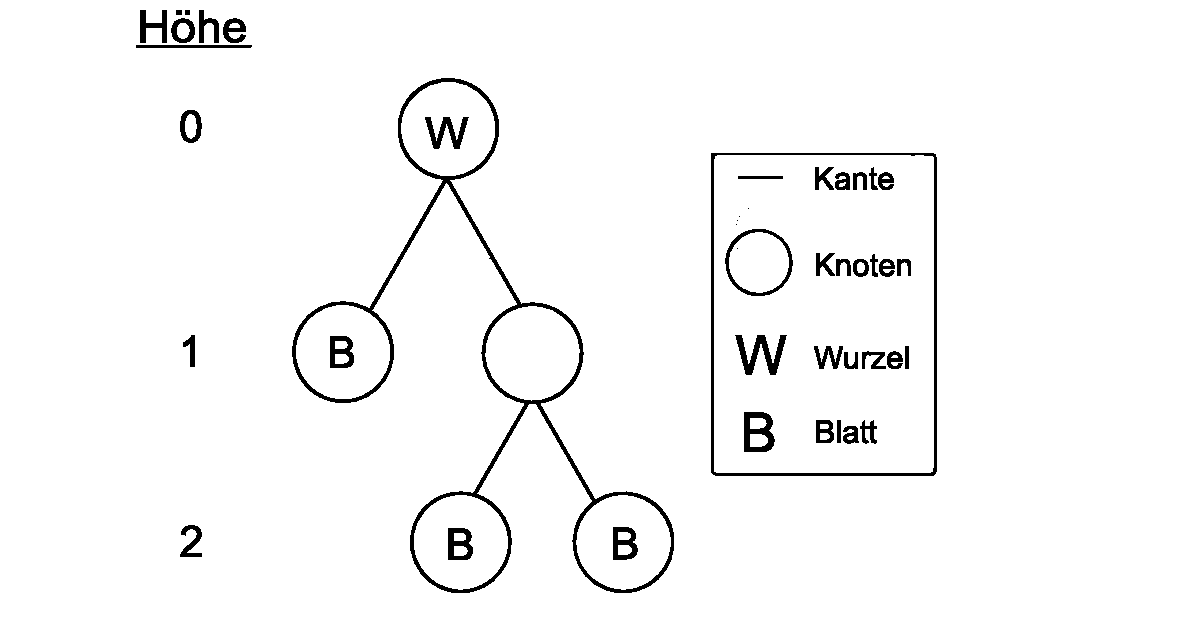
\includegraphics[scale = 0.5]{abbildungen/simple_tree}
    \caption{Einfacher beschrifteter Binärbaum}
    \label{pic:simple_tree} 
\end{figure}

Eine spezielle Form von Bäumen stellen die sogenannten Binärbäume dar. 
Binärbäume sind Bäume, wo jeder Knoten maximal zwei Kinder hat. Abbildung \ref{pic:simple_tree} 
zeigt einen einfachen Binärbaum, wo jedes Element genau beschriftet ist. 

Um jeden Knoten eines Baumes abarbeiten zu können, kann über dem Baum 
traversiert werden. Traversierung bezeichnet das systematische Ablaufen 
von jedem Knoten eines Baumes. Der naive Algorithmus
von Wetherell und Shannon verwendet die sogenannte
Pre-Order-Traversierung. Dabei wird zunächst der Knoten, dann der linke Teilbaum
und zum Schluss der rechte Teilbaum besucht. Hier werden die Väter also vor den
Kindern durchlaufen. Sowohl der verbesserte Algorithmus von Wetherell 
und Shannon als auch der Algorithmus von Reingold und Tilford verwenden hingegen die 
Post-Order-Traversierung. Dabei wird als erstes der linke Teilbaum, dann der 
rechte Teilbaum und dann der Knoten besucht \cite[]{q4}. Bei dieser Art der 
Traversierung werden die Kinder also vor den Väter durchlaufen. Neben diesen Arten
der Traversierung gibt es noch weitere Möglichkeiten, wie über einem 
Baum traversiert werden kann. Diese sind für das Verständnis der hier 
vorgestellten Algorithmen aber nicht notwendig.


\section{Anwendungsgebiete}

Bäume erfahren einen vielfältigen Einsatz in der Informatik, zum Beispiel 
als Datenstruktur, als Syntaxbäume, als Ausdrucksbäume oder auch als 
Entscheidungsbäume.

Ein Baum als Datenstruktur kann beispielsweise dazu verwendet werden, 
um eine Menge von Daten zu sortieren oder in ihnen effizient nach einen 
bestimmten Datensatz zu suchen. So verwendet der Heap-Sort-Algorithmus 
einen Baum zum Sortieren von Daten. Ebenso können Bäume dazu verwendet 
werden, die Syntax von Quellcode zu überprüfen. Ferner werden diese Bäume 
als Syntaxbäume bezeichnet. Zudem werden Bäume verwendet um mathematische 
Ausdrücke auszuwerten. Hierfür wird ein sogenannter Ausdrucksbaum für einen 
gegebenen mathematischen Ausdruck aufgestellt und ausgewertet. In der 
Datenanalyse werden Bäume in Form von Entscheidungsbäumen verwendet. 
Diese werden benutzt um Abhängigkeiten darzustellen. Die Blätter stellen 
Kategorien dar und die Knoten Bedingungen. So können beispielsweise neue 
Datensätze, in Abhängigkeit zu seinen Werten, einer bestimmten Kategorie 
zugeordnet werden.

Auch außerhalb der Informatik werden Bäume häufig verwendet. Sie können 
dazu verwendet werden um zum Beispiel eine Hierarchie eines Unternehmens 
(siehe Abb. 1) dazustellen oder einen Stammbaum einer 
Familie (siehe Abb. 2) \cite[]{q4}.

\todo{Zwei beispielhafte Abbildungen erstellen}


\chapter{Algorithmen zum Zeichnen von Bäumen}
\label{chap:kapitel3}

\section{Naiver Algorithmus von Wetherell und Shannon}

Das Paper “Tidy Drawings of Trees” von Charles Wetherell und Alfred Shannon aus dem Jahre 1979, 
welches im IEEE Trans. Softw. Eng. erschienen ist, handelt von verschiedenen Algorithmen zum Zeichnen von Bäumen.
Der erste Algorithmus, der von den beiden Autoren beschrieben und vorgestellt wird, ist ein naiver Algorithmus 
zum Zeichnen von Bäumen. Dieser Algorithmus soll dabei zwei Anforderungen erfüllen. Die erste Anforderung wird dabei
an die Ästhetik des gezeichneten Baumes gestellt. Alle Knoten, die dieselbe Höhe haben, sollen sich auf einer horizontalen
Linie befinden. Jede Höhe hat dabei eine Linie, auf welcher sich die Knoten befinden sollen und diese Linien sollen alle
parallel zueinander sein. Außerdem soll der Algorithmus beim Zeichnen eines Baumes ein physikalisches Limit einhalten.
Das bedeutet, dass der Algorithmus möglichst schmale Bäume zeichnen soll. Jedoch wird die Höhe des Baumes durch diese Anforderungen
nicht eingeschränkt. Stattdessen bestimmt der Baum selbst seine Höhe. \cite[]{q1}

\subsection{Ablauf}
Bevor die Funktionsweise des Algorithmus beschrieben werden kann, muss die Baumstruktur wie folgt definiert sein: Sie benötigt eine Struktur die symbolisch für ein Knoten des Baums steht. Diese Knoten-Struktur muss hierbei ihren Vater kennen, auf ihre Kinder zugreifen können, ihre Position speichern können. Diese Hilfsvariable wird dazu benutzt, um das nächste abzuarbeitende Kind eines Knoten zu identifizieren. 

In Java könnte diese Struktur beispielsweise wie folgt aussehen:
\begin{lstlisting}
class Knoten {
	Knoten vater;
	Knoten[] kinder;
	int hoehe;
	int x, y;
}
\end{lstlisting}
Dieser Algorithmus besitzt zwei Eingabeparameter: Die Wurzel und Höhe des Baumes. Die Wurzel muss hierbei vom Typ der zuvor definierten Struktur sein. Zu Beginn wird eine Variable definiert: Ein Array (später Positions-Array genannt), die die jeweils nächst freie X-Position einer Ebene des Baums beinhaltet. Hiernach wird über die Baumstruktur der Wurzel, in der Pre-Order-Traversierung, traversiert. Nun werden die X und Y Attribute der Knoten wie folgt bestimmt und gesetzt:

Der derzeitige Knoten bekommt als X-Position den Wert aus dem Positions-Array, in Abhängigkeit von seiner Höhe im Baum. Hiernach wird die Zahl im Positions-Array inkrementiert. Die Y-Position des Knoten wird nun in Abhängigkeit zur Höhe des Knoten mit der folgenden Formel berechnet: y := 2 * Höhe + 1.

Dieses Vorgehen wird nun für alle Knoten in dem Baum wiederholt. 

Nach dem Durchlaufen aller Knoten des Baumes sind alle X und Y-Koordinate gesetzt und der Baum kann gezeichnet werden.

\subsection{Vor- und Nachteile}

\section{Verbesserter Algorithmus von Wetherell und Shannon}

\subsection{Ablauf}

\subsection{Vor- und Nachteile}

\section{Algorithmus von Reingold und Tilford}

\subsection{Ablauf}

\subsection{Implementierung in Java}

\subsection{Vor- und Nachteile}

\subsection{Modifizierung des Algorithmus}


\chapter{Analyse vorhandener Daten}
\label{chap:kapitel4}

Ein Modell, welches beim Data Mining genutzt werden kann, ist das \ac*{CRISP-DM}. Diese Modell definiert das Data Mining als Prozess mit sechs verschiedenen Phasen und kann der 
Abbildung \ref*{fig:CRISP-DM} entnommen werden. Dabei dürfen diese Phasen nicht als starr aufeinander folgend betrachtet werden. Denn auch Erkenntnisse aus nachfolgende Phasen können vorherige Phasen
beeinflussen, was deutlich wird, durch die Pfeile zwischen den Phasen in der Abbildung \ref*{fig:CRISP-DM}. In der ersten Phase, dem Business Understanding, liegt der Schwerpunkt auf dem Verständnis 
der Projektziele aus der Geschäftsperspektive. Mit dem erlangten Wissen daraus, kann eine Data-Mining Problemstellung definiert werden, wie dies in Kapitel \ref*{chap:Zielsetzung} erfolgt ist. 
Die nächste Phase ist das Data Understanding. Diese Phase beschäftigt sich mit der ersten Datenerhebung und dem Aufbau eines Datenverständnisses. Zudem wird in dieser Phase versucht mögliche Probleme 
bei der Qualität der Daten zu identifizieren. Nach der Phase des Data Understandings folgt die Phase der Data Preparation. Während dieser Phase ist das Ziel die Rohdaten so aufzubereiten, dass ein 
Datensatz dabei erstellt wird, der für eine Modellierung geeignet ist \cite[S.5-7]{q8}. Die nächsten drei Phasen beschäftigen sich mit der Modellierung, der Evaluierung von Modellen und dem Einsatz 
eines Modells und gehen somit über die Aufgabenstellung des Praxisprojekt hinaus und werden deshalb im Folgenden nicht berücksichtigt.

\begin{figure}[H]
    \centering
    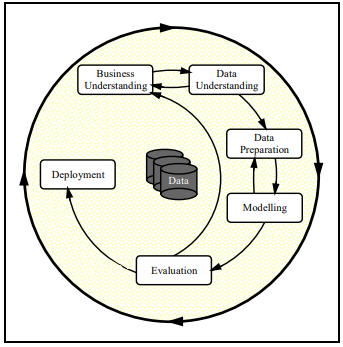
\includegraphics[]{abbildungen/CrispDM.PNG}
    \caption{\ac*{CRISP-DM} Phasen \cite[S.5]{q8}}
    \label{fig:CRISP-DM}
\end{figure}



\section{Data Understanding}
\label{chap:DataUnderstanding}

In der Baumansicht auf der linken Seite der Abbildung \ref*{fig:Doors GUI} befindet sich ein Projekt mit dem Namen \glqq RA Application Conditions\grqq{}. In diesem Projekt befinden sich Module, welche
Anwendungsregeln von diversen Komponenten beinhalten. Dafür wurde ein Script in \acs{DXL} geschrieben, welches über alle Module innerhalb des Projekts iteriert. Wenn das aktuelle Element ein Modul ist,
muss dieses geöffnet werden und falls dieses nicht NULL ist muss über jedes Objekt in diesem Modul iteriert werden. Bei jedem Objekt muss daraufhin über alle In-Links iteriert werden. Über diese 
In-Links ist es möglich das Quellmodul zu bestimmen, also das Modul, von dem der Link kommt. Diese Quellmodule sind potentiell relevante Module für das Anlernen des KI-Systems. Nach dem Process Manual für
Anwendungsregeln der Siemens Mobility GmbH \cite[S.32]{q2} muss das Link-Modul des Links den Namen \glqq 42\char95 reference\char95 of\grqq{} tragen. Bei älteren Projekten jedoch wurde als Name 
\glqq reference\char95 of\grqq{} genutzt. Zudem kann der Fall auftreten, dass Quellmodule in einer Sandbox eines Mitarbeiters liegen. Diese Module dürfen nicht berücksichtigt werden, da sie kein Teil
von Projekten der Siemens Mobility GmbH sind. Alle Quellmodule, die den Anforderungen entsprechen, werden in eine Skiplist eingefügt. Skiplisten sind eine Datenstrukturen, welche aus einem 
Key-Value-Paar bestehen. 

\begin{lstlisting}[caption={Iterieren über alle Module von RA Application Conditions},captionpos=b, label = lst:searchInLinks]
Folder f = folder("/RA Application Conditions");
void searchInLinks(Folder f){
    for it in f do{
        if (type(it) == "Folder"){
            searchInlinks(folder(it));
        }
        if (type(it) == "Formal"){
            m = read(fullName it, false);
            if (m != null){
                for o in entire m do{
                    for lr in all (o <- "*") do {
                        if (name module lr == "42_reference_of" 
                        || name module lr == "reference_of") {
                            srcModRef = source lr;
                            iOffset = null;
                            iLength = null;
                            if(!(findPlainText(fullName srcModRef, 
                            "Sandbox", iOffset, iLength, false))){
                                put(slModules, fullName srcModRef, 
                                fullName srcModRef);
                                // ...
\end{lstlisting}

Nach dem Iterieren aller Module im Projekt RA Application Conditions lassen sich 115 Module aus 63 Projekten finden, welche einen Link zu Anwendungsregeln besitzen und diese somit importiert haben.
Diese Projekte mit ihren Modulen sind potentielle Kandidaten für einen Datensatz zum Anlernen des KI-Systems. Als nächsten Schritt müssen diese Module genauer betrachtet werden. Es muss geprüft werden,
welche Attribute für das Bewerten von Anwendungsregeln relevant sind. Der Quellcode \ref*{lst:getAttribute} zeigt eine Möglichkeit, sich alle Attribute eines Moduls ausgeben zu lassen. 
Nach dem Process Manual für Anwendungsregeln müssen Projekte, welche Anwendungsregeln importiert haben, die Attribute REQ Status und REQ Statement beinhalten. Das Attribut REQ Status vom Typ einer
single-enumeration beinhaltet dabei die Bewertung der Anwendungsregel. Die Begründung dafür lässt sich im Attribut REQ Statement in Textform finden\cite[S.14]{q2}. 


\begin{lstlisting}[caption={Alle Attribute eines Moduls ausgeben \cite{q9}}, captionpos=b, label = lst:getAttribute] 
string modAttrName
for modAttrName in attributes (current Module) do
    print modAttrName "\n"
\end{lstlisting}

Die folgende Aufzählung beinhaltet eine Auswahl von Attributen eines beispielhaft gewählten Moduls. 

\begin{multicols}{3}
    \begin{itemize}
        \setlength{\itemsep}{0cm}
        \item Absolute Number
        \item ALinkRef
        \item Compare
        \item Last Modified On
        \item Object Heading
        \item Object Short Text
        \item Object Text
        \item OLE
        \item OLEIconic
        \item Picture
        \item PictureName
        \item PictureNum
        \item REQ Comment\char95 int
        \item REQ Domain
        \item REQ Statement
        \item REQ Status
        \item REQ Type
        \item RTF Pict
        \item STD Explanation
        \item STD Identifier
        \item STD Title
    \end{itemize}
\end{multicols}

Für das Bewerten der Anwendungsregel ist der Object Text, also die Anwendungsregel in Textform, sowie die Attribute REQ Statement und REQ Status relevant, da das KI-System später Vorschläge
für diese beiden Attribute liefern soll. Die Analyse von Modulen von Projekten, 
welche vor 2016 durchgeführt wurden, hat gezeigt, dass dort das Attribut REQ Status den Namen REQ Progress trägt. Darauf muss bei dem Sammeln der Daten und der späteren Aufbereitung dieser geachtet
werden. Zudem wurde dabei deutlich, dass einige Module weder REQ Status bzw. REQ Progress noch REQ Statement als Attribut besitzen. Mögliche Erklärungsansätze dafür wären, dass die Projektausführung
von den Vorgaben des Process Manuals abweichen, dass die Projekte sich noch in einem frühen Stadium befinden und deshalb die Anwendungsregeln nicht bewertet wurden oder dass die Anwendungsregeln lediglich
importiert, aber nicht bewertet wurden.

Außerdem muss beachtet werden, dass ein Projekt mittels eines Copy-Update-Tools die Anwendungsregeln auf eine neue Version updaten kann. Die alten Versionen der Anwendungsregeln werden dann unter ein Objekt
verschoben, welches die Überschrift \glqq Old Version Objects, to be reviewed and deleted: \grqq{} hat. Diese Anwendungsregeln dürfen nicht verwendet werden, da diese veraltet sein können. 

\section{Data Preparation}

Mit den Erkenntnissen aus der vorherigen Phase beginnt nun die Aufbereitung der Daten. Jede Komponente bzw. jedes System hat im Project RA Application Conditions einen Ordner \glqq 10\char95 Project
Answers\grqq{}. Nutzt ein Projekt nun beispielsweise das Achszähler-System AzS350U und hat die Anwendungsregeln des Systems bewertet, dann müssen diese bewerteten Anwendungsregeln in ein neues Modul 
in dem \glqq 10\char95 Project Answers\grqq{} Ordner des Achszähler-Systems geschrieben werden. Mit den Modulen, die die bewerteten Anwendungsregeln der einzelnen Komponenten und Systeme beinhalten,
kann dann das KI-System angelernt werden. 

Um das zu erreichen, müssen zunächst die 115 Module genauer untersucht werden. Dabei muss geprüft werden, ob diese Module die Anwendungsregeln so bewertet haben, wie es das Process Manual vorgibt.
Dafür muss die Iteration aus \ref*{lst:searchInLinks} erweitert werden. Es muss zusätzlich geprüft werden, ob das Modul die Attribute REQ Status bzw. REQ Progress besitzt und ob diese auch 
ausgefüllt sind. 

\begin{lstlisting}[caption={Suche nach bewerteten Anwendungsregeln},captionpos=b, label = lst:searchARSolutions]                                                       
if(hasAttribute("REQ Status", mod) 
&& hasAttribute("REQ Statement", mod)){  
    szProgress = o."REQ Status""";
    szStatement = o."REQ Statement";
    if(length(szProgress)>1 && length(szStatement)>1){ 
        put(slResults, fullName mCheck, fullName mCheck)
    }
}else if (hasAttribute("REQ Progress", mod) 
&& hasAttribute("REQ Statement", mod)){
    szProgress = o."REQ Progress""";
    szStatement = o."REQ Statement";
    if(length(szProgress)>1 && length(szStatement)>1){ 
        put(slResults, fullName mCheck, fullName mCheck)
        // ...
\end{lstlisting}

Übrig bleiben danach 41 Module aus 34 Projekten, welche nicht nur die Anwendungsregeln importiert, sondern auch nach den Vorgaben des Process Manuals bewertet haben. Als Zwischenschritt wurde daraufhin
für jedes Projekt ein Modul in meiner Sandbox erstellt. In diesem Modul wurden dann alle bewerteten Anwendungsregeln reingeschrieben. Dabei musste darauf geachtet werden, dass auschließlich die
Anwendungsregeln in das Modul geschrieben wurden und keine Überschriften oder Ähnliches. Zudem durften nur die relevanten Attribute in dem neuen Modul stehen. Alle weiteren Attribute dürfen nicht
hinzugefügt werden, da diese für das Bewerten von Anwendungsregeln irrelevant sind und die Module und somit den schlussendlichen Datensatz, welcher zum Trainieren des KI-Systems verwendet werden soll,
unnötig groß machen würden. Zudem muss, wie in Kapitel \ref*{chap:DataUnderstanding} beschrieben, überprüft werden, ob sich die Anwendungsregel unter dem Punkt 
\glqq Old Version Objects, to be reviewed and deleted: \grqq{} befindet. Dafür muss über alle Väter eines Objekts iteriert werden und geprüft werden, ob die Überschrift eines Objekts 
\glqq Old Version Objects, to be reviewed and deleted: \grqq{} ist. Der Quellcode \ref*{lst:checkOld} zeigt eine Möglichkeit, bei der eine Boolean-Variable auf true gesetzt wird, falls ein Objekt
veraltet ist. Diese Objekte werden dann nicht in das neue Modul geschrieben.

\begin{lstlisting}[caption={Prüfen, ob Objekt veraltet ist}, captionpos=b, label = lst:checkOld] 
for obj in entire mod do{ 
    oParent = parent(obj)
    bOldVersion = false;
    while (oParent != null){
        if (oParent."Object Heading""" ==  "Old Version Objects, to be reviewed and deleted:"){
            bOldVersion = true;
        }
        oParent = parent(oParent)
    }
\end{lstlisting}

Abbildung \ref*{fig:SolutionsModul} zeigt, wie ein Modul für ein Projekt dann aussieht. Erkennbar ist, dass dort lediglich die relevanten Attribute gespeichert werden. Zudem wird ein Out-Link auf die
Anwendungsregel unter RA Application Conditions gesetzt, damit nachverfolgt werden kann, von wo die Anwendungsregel ursprünglich stammt. Des Weiteren besteht der Name des Moduls aus dem Namen
des Projekt sowie der Endung \glqq \char95 Solutions\grqq{}. Dadurch wird sichergestellt, dass die Information darüber, von welchem Projekt die bewertete Anwendungsregel stammt, erhalten bleibt.

\begin{figure}[H]
    \centering
    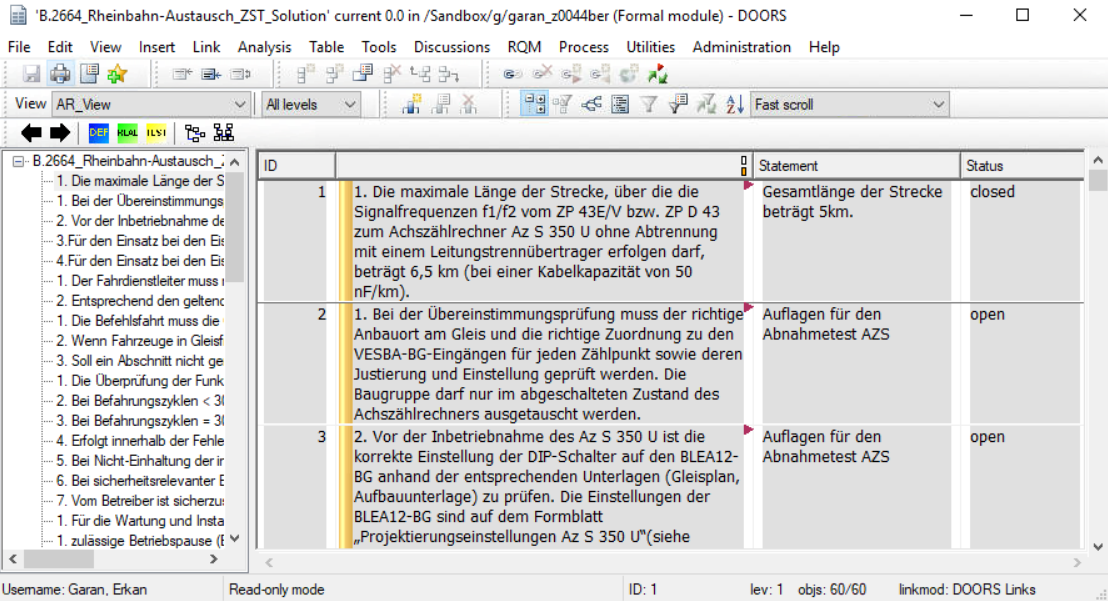
\includegraphics[width = \textwidth]{abbildungen/Solutions.PNG}
    \caption{Modul eines Projekts}
    \label{fig:SolutionsModul}
\end{figure}



% TODO

- Zwischenschritt: für jedes Projekt ein Modul in Sandbox
- dabei darauf achten, dass nur relevante Attribute kopiert werden und keine old versions
- diese dann aufteilen, auf einzelne Komponenten/Systeme durch Links
- die neuen Module dann in Projects Answers einfügen
- FERTIG

\chapter{Modellierung}
\label{chap:Modellierung}
Dieses Kapitel wird sich mit der Erstellung eines \ac{KI}-Modells als \ac{NN} mithilfe der Keras-Bibliothek in Python beschäftigen. Dabei werden die verschiedenen Möglichkeiten
zur Modellierung des Modells vorgestellt, erläutert und diskutiert. Zum Schluss wird gezeigt, wie so ein Modell verwendet werden kann und wie gut es seine Aufgabe lösen kann.

\section{Definieren des ersten neuronalen Netzes}
\label{chap:DefineNN}
Nachdem der Trainingsdatensatz definiert und in Ein- und Ausgabewerte aufgeteilt wurde, muss als Nächstes das \ac{NN} definiert werden, wie es Kapitel \ref{chap:Keras} beschriebt.
Dafür bietet die Keras-Bibliothek die Klasse \glqq Sequential\grqq{}, die genutzt werden kann, wenn Schichten sequentiell angeordnet werden sollen. Laut Chollet ist diese Art der 
Netzarchitektur die am häufigsten genutzte \cite[vgl. S.92]{DL_PY}. 

\begin{lstlisting}[language = python, caption={Erstellung eines sequentiellen Modells},captionpos=b, label = lst:ModellSeq, floatplacement=H]
    from keras.models import Sequential
    from keras.layers import Dense
    from keras.losses import CategoricalCrossentropy 

    model = Sequential()
    model.add(Dense(8, input_shape=(trainX.shape[1],), activation='relu'))
    model.add(Dense(16, activation='relu'))
    model.add(Dense(trainYStatus.shape[1], activation='softmax'))
\end{lstlisting}

Der Quellcode \ref{lst:ModellSeq} zeigt die benötigten Imports und wie ein Modell zur Vorhersage des Statuswerts definiert werden kann. Zuerst wird ein Objekt vom Typ Sequential erstellt. Diesem Objekt 
können dann die verschiedenen Schichten hinzugefügt werden. Dabei muss bestimmt werden, wie viele Schichten das Modell haben soll und wie viele Neuronen jede Schicht besitzen soll.
Als erste Schicht wird eine Dense-Layer als Eingabeschicht mit acht Neuronen definiert. Eine Dense-Layer ist eine fully-connected Schicht,
wie beispielsweise die Schichten in der Abbildung \ref{fig:NN_Modell}, und erwartet als Parameter mindestens die Anzahl an Neuronen. Optional können noch weitere Parameter angegeben werden.
Die Eingabeschicht benötigt als Besonderheit noch zusätzlich die Anzahl an Attributen, diese können dem Dataframe mit den Eingabewerten entnommen werden. Als Aktivierungsfunktion wird
die \ac{ReLU}-Funktion genutzt, die bereits in Kapitel \ref{chap:DL} vorgestellt wurde und auch die verbreitetste Aktivierungsfunktion beim \ac{DL} ist \cite[vgl. S.102]{DL_PY}. 
Als erste versteckte Schicht wird eine weitere Dense-Layer genutzt, hier mit 16 Neuronen. 
Die Anzahl an Neuronen und die Tiefe des Modells bestimmt die Komplexität des Modells. Ein zu komplexes Modell kann zu Überanpassung und ein zu simples Modell zu Unteranpassung führen.
Im Vorhinein ist es schwierig die benötigte Komplexität zu bestimmen, weshalb die Anzahl an Schichten und Neuronen, in Abhängigkeit zu dem Ergebnis des Modells, im Laufe der Erstellung noch geändert 
werden sollten. Als letzte Schicht und somit als Ausgabeschicht wird ebenfalls eine Dense-Layer verwendet. Die Anzahl an Neuronen in der Ausgabeschicht ist abhängig von der Anzahl an 
möglichen Ausprägungen des zu bestimmenden Wertes. Die ausgewählte Anwendungsregel wurde in der Vergangenheit mit \glqq closed\grqq{}, \glqq compliant\grqq{} und \glqq not applicable\grqq{} bewertet,
weshalb in diesem Fall die Ausgabeschicht drei Neuronen besitzen muss. Jedes Neuron stellt dabei eine mögliche Ausprägung dar. Anders als bei den vorherigen Schichten wurde bei dieser Schicht 
als Aktivierungsfunktion \glqq Softmax\grqq{} gewählt. Diese Aktivierungsfunktion weist jedem Neuron eine Wahrscheinlichkeit zwischen null und eins zu, wobei die Summe aller Wahrscheinlichkeiten 
eins ergibt \cite{KerasDoc}. Diese Eigenschaft der Funktion ist auch der Grund, weshalb für Status und Statement eigene Modelle erstellt werden müssen, da das Sequential-Modell nur eine Ausgabeschicht
erlaubt und es somit nicht möglich ist, mit dieser Funktion zwei Kategorien vorherzusagen. 

Die Auswahl der Aktivierungsfunktion der Ausgabeschicht ist abhängig von der Aufgabe des Modells. 
\glqq Softmax\grqq{} bietet sich zum Beispiel ideal als Möglichkeit zur Klassifikation an, wenn mehrere verschiedene Klassifizierungen vorhanden sind. Wenn nur zwei verschiedene Zustände möglich sind, 
also ein binäres Klassifikationsproblem vorliegt, würde sich als Aktivierungsfunktion eine Sigmoidfunktion anbieten, da diese beliebige Werte einen Ausgabebereich zwischen null und eins 
zuordnet \cite[vgl. S.100]{DL_PY}.

\begin{lstlisting}[language = python, caption={Zusammenfassung des Modells},captionpos=b, label = lst:ModellSummary, float, floatplacement=H]
    model.summary()
    ---------------------------------------
    Output:
    Model: "sequential"
    _______________________________________________________________
    Layer (type)                Output Shape              Param #   
    ===============================================================
    dense (Dense)               (None, 8)                 1424      
                                                                    
    dense_1 (Dense)             (None, 16)                144       
                                                                    
    dense_2 (Dense)             (None, 3)                 51        
                                                                    
    ===============================================================
    Total params: 1,619
    Trainable params: 1,619
    Non-trainable params: 0
    _______________________________________________________________
\end{lstlisting}
Eine Zusammenfassung wurde mit der summary()-Methode im Quellcode \ref{lst:ModellSummary} ausgegeben. 
Diese Zusammenfassung zeigt nochmal die verschiedenen Schichten, die Dimension der Ausgabe der Schichten sowie die Anzahl an Parametern in jeder Schicht an. 
Zu erkennen sind dort die drei hinzugefügten Dense-Layer. Die erste Dimension der Ausgabe ist \glqq None\grqq{}, da die Anzahl an Einträgen vorher nicht festgelegt wurde. 
Die zweite Dimension wird bestimmt durch die Anzahl an Neuronen in einer Schicht.\\

Je nach Anwendungsfall würden andere Schichten als die Dense-Layer infrage kommen. Stehen die Daten in einem sequentiellen Zusammenhang, beispielsweise eine Zeitreihe von Wetterdaten, dann würden
die sogenannten LSTM-Layer infrage kommen. LSTM steht für Long Short-Term-Memory(auf Deutsch: langes Kurzzeitgedächtnis) und diese Art von Schicht ist in der Lage Informationen mehrere Zeitschritte
lang zu erhalten \cite[vgl. S.260]{DL_PY}. Bei der Computer Vision werden häufig CNNs (Convolutional Neuronal Networks) genutzt. Ein CNN besteht dabei nicht aus Dense-Layern, wie in diesem 
Anwendungsfall, sondern aus Convolutional-Layern. Diese Schichten können zum Beispiel lokale Muster in Bildern erlernen und diese in neuen Bildern wiedererkennen, auch wenn sie nicht an derselben Stelle
sind \cite[vgl. S.164]{DL_PY}. Diese Schichten werden also in anderen Anwendungsfällen genutzt, für diesen Anwendungsfall eignen sich jedoch die Dense-Layer am besten.    \\

Bevor das Modell mit den Daten angelernt werden kann, müssen zunächst noch die Verlustfunktion und ein Optimierer ausgewählt werden. Da der Aufgabentyp eine Single-Label-Mehrfachklassifizierung 
ist, also eine Klassifizierung wo eine Klasse aus mehreren Klassen gewählt werden muss, wird als Verlustfunktion die kategorische Kreuzentropie genutzt. 
Eine Kreuzentropie misst die Differenz zwischen den vorhergesagten Wahrscheinlichkeiten und dem tatsächlichen Wert \cite[vgl. S.102]{DL_PY}.
Bei der kategorischen Kreuzentropie wird erwartet, dass die Ausgabewerte in der One-Hot-Codierung vorliegen. Sind die Ausgabewerte mit dem Label-Encoding codiert,
müsste als Verlustfunktion die \glqq Sparse Categorical Crossentropy\grqq{} genutzt werden \cite{KerasDoc}. Für andere Aufgabentypen werden andere 
Verlustfunktionen genutzt. Zum Beispiel bei einer Regression bietet sich der mittlere quadratische Fehler an oder bei der Binärklassifizierung die binäre Kreuzentropie \cite[vgl. S.155]{DL_PY}.
Während des Trainings wird das Modell versuchen das Ergebnis der kategorischen Kreuzentropie zu minimieren. 

Als Optimierer soll, laut Chollet, in den meisten Fällen der \glqq rmsprop\grqq{}-Optimierer mit der voreingestellten Lernrate verwendet werden können \cite[vgl. S.155]{DL_PY}. Ähnlich wie bei 
der Komplexität des Modells ist es schwierig vorher genau zu bestimmen, welcher Optimierer für die spezifische Anwendung die besten Ergebnisse liefert. Deshalb muss auch hier ausprobiert werden.
Zunächst wird sich an die Empfehlung von Chollet gehalten, es existieren jedoch auch weitere Optimierer, wie zum Beispiel \glqq Adam\grqq{} oder \glqq SGD\grqq{}, die berücksichtigt 
werden sollten \cite{KerasDoc}. 

Die Verlustfunktion sowie der Optimierer können nun, wie im Quellcode \ref*{lst:ModelCompile} gezeigt, ausgewählt werden. Diese werden der compile()-Methode als Parameter übergeben.
Zudem muss noch eine Kenngröße ausgewählt werden, die während des Anlernens überwacht wird. In diesem Fall wird dafür die \glqq categorical\_accuracy\grqq{} verwendet.
Diese Kenngröße gibt an, wie oft Vorhersagen den One-Hot codierten Ausgabewerten entsprechen.

\begin{lstlisting}[language = python, caption={Auswahl des Optimierers sowie der Verlustfunktion},captionpos=b, label = lst:ModelCompile, float, floatplacement=H]
    model.compile(optimizer='rmsprop',
        loss=CategoricalCrossentropy(),
        metrics=['categorical_accuracy'])
\end{lstlisting}

Nun ist das Modell fertig konfiguriert und kann auf den Trainingsdaten trainiert werden.

\subsection{Training des Modells}
\label{chap:TrainNN}

Zum Trainieren des Modells mit den vorher definierten und codierten Daten wird die fit()-Methode genutzt. Dieser Methode werden die Ein- und Ausgabewerte übergeben, mit dem das Modell trainiert werden soll.
Weitere Parameter sind:
\begin{description}[style=multiline,leftmargin=4cm,font=\bfseries, nolistsep]
    \item[batch\_size] Anzahl an Trainingsbeispielen, bevor die Gewichte des \ac{NN}~geupdatet werden \cite{KerasDoc}
    \item[epochs] Anzahl an Iterationen über den gesamten Trainingsdatensatz \cite{KerasDoc}
    \item[verbose] Bestimmt die Menge an Terminalausgaben \cite{KerasDoc}
    \item[validation\_split] Anteil des Trainingsdatensatzes, der zum Testen benutzt werden soll \cite{KerasDoc}
\end{description} 
Quellcode \ref*{lst:TrainModel} zeigt, wie hier die Parameter definiert wurden. In diesem ersten Trainingsansatz wurde als \glqq batch\_size\grqq{} zwei gewählt, was bedeutet, dass das Modell
nach jedem zweiten Trainingsbeispiel die Gewichte des Modells ändert. Da die ausgewählte Anwendungsregel lediglich 17-Mal bewertet wurde, muss die \glqq batch\_size\grqq{} dementsprechend niedrig gewählt
werden. Je niedriger die \glqq batch\_size\grqq{} ist, desto genauer kann das Modell die Trainingsdaten erlernen, was jedoch auch zu Overfitting führen kann. Zudem kann ein niedrigerer Wert 
die Laufzeit des Trainingsprozesses negativ beeinflussen, da das Modell häufiger geupdatet werden muss.

Die Anzahl an zu durchlaufenden Epochen wurde zunächst mit 50 gewählt. Hier muss ebenfalls im Nachhinein geprüft werden, wie viele Epochen benötigt werden. Eine höhere Anzahl an Epochen kann zu 
Overfitting führen, eine zu niedrige Anzahl zu Underfitting. Hier muss also mithilfe der Kenngröße geprüft werden, wie sich das Modell mit zunehmender/abnehmender Anzahl an Epochen verhält.

Für den Parameter \glqq verbose\grqq{} wurde der Wert zwei gewählt. Dieser sorgt dafür, dass die maximale Menge an Terminalausgaben ausgegeben wird. Ein Wert von eins würde nur einen 
Fortschrittsbalken ausgeben, ein Wert von null würde gar keine Ausgabe produzieren \cite{KerasDoc}.

Da ein Datensatz niemals mit den Trainingsdaten getestet werden sollte, muss eine Aufteilung in Testdaten erfolgen. Wie in Kapitel \ref*{chap:Trainingssplit} erwähnt, kann der Testsplit
während des Anlernens erfolgen. Dafür bietet Keras die Möglichkeit automatisch einen Teil der Trainingsdaten zum Testen zu benutzen.
In diesem Fall werden 25~\% des Datensatzes als Testdaten verwendet. Bei 17 Einträgen wären das 4,25 Einträge, die aber aufgerundet werden, also werden fünf Einträge 
nicht zum Trainieren benutzt, sondern werden fürs Testen zurückgehalten.

\begin{lstlisting}[language = python, caption={Trainieren des Modells},captionpos=b, label = lst:TrainModel, float, floatplacement=H]
    history = model.fit(trainX, trainYStatus,
                    batch_size=2,
                    epochs=50,
                    verbose=2,
                    validation_split=0.25)
\end{lstlisting}

\subsection{Testen des Modells}
\label{chap:TestNN}

Die Ausgabe des Trainingsprozesses kann dabei der Abbildung \ref*{fig:TrainModel} entnommen werden. Da der \glqq verbose\grqq{}-Wert auf zwei gesetzt wurde, wird für jede Epoche eine Ausgabe
generiert. Diese Ausgabe beinhaltet die benötigte Zeit für jede Epoche sowie den Wert der Verlustfunktion und der gewählten Kenngröße für die Trainings- und Testdaten.
\begin{figure}[H]
    \centering
    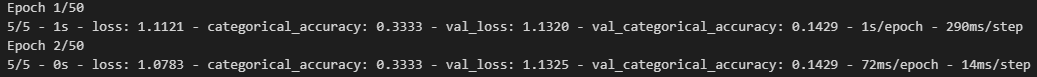
\includegraphics[width = \textwidth]{abbildungen/TrainAusgabe.png}
    \caption{Ausgabe des Trainingsprozesses}
    \label{fig:TrainModel}
\end{figure}
Der Wert der Verlustfunktion sowie die Genauigkeit können auch zusätzlich visualisiert werden, um den Verlauf darzustellen. Dazu wird das Objekt genutzt, welches bei Aufruf der 
fit()-Methode im Quellcode \ref*{lst:TrainModel} zurückgegeben und in der Variable \glqq history\grqq{} gespeichert wurde. Dieses Objekt beinhaltet 
den Wert der Verlustfunktion und die Genauigkeit für die Trainings- und Testdaten. Mithilfe der Matplotlib-Bibliothek können diese Werte dann in einem Liniendiagramm visualisiert werden,
der Quellcode \ref*{lst:PlotLoss} zeigt die benötigten Schritte für das Erstellen eines Liniendiagramms für die Verlustfunktion, die Genauigkeit kann jedoch äquivalent dazu 
dargestellt werden. Neben der Übergabe der Daten und der dazugehörigen Label können auch ein Titel und eine Achsenbeschriftung hinzugefügt werden, wie Zeile drei und vier des Quellcodes zeigen.
\begin{lstlisting}[language = python, caption={Trainieren des Modells},captionpos=b, label = lst:PlotLoss, float, floatplacement=H]
    plt.plot(history.history['loss'], label = 'Training loss')
    plt.plot(history.history['val_loss'], label = 'Validation loss')
    plt.title('Wert der Verlustfunktion')
    plt.xlabel('Epochen')
    plt.legend()
\end{lstlisting}
Abbildungen \ref*{fig:plotLoss} und \ref*{fig:plotAcc} zeigen die beiden erstellten Diagramme. Dort ist zu erkennen, dass mit zunehmender Anzahl an Epochen der Wert der Verlustfunktion abnimmt,
während die Genauigkeit zunimmt, was ein idealer Fall wäre. Die Werte sind jedoch mit Vorsicht zu betrachten, da sie nur ein Beispiel für ein Modell darstellen.
Da der Datensatz sehr klein ist, kann es sein, dass zufällig Testdaten ausgewählt wurden, die das Modell leichter erkennen konnte, bei erneuter Ausführung könnten die 
Werte deshalb stark schwanken.

\begin{figure}[H]
    \centering
    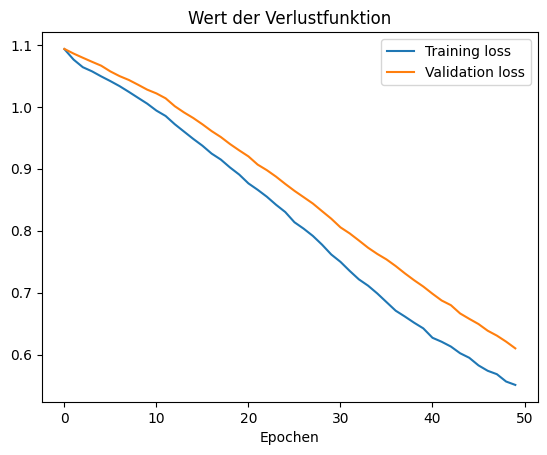
\includegraphics[width=.75\textwidth]{abbildungen/PlotLoss.png}
    \caption{Plot der Verlustfunktion}
    \label{fig:plotLoss}
\end{figure}
\begin{figure}[H]
    \centering
    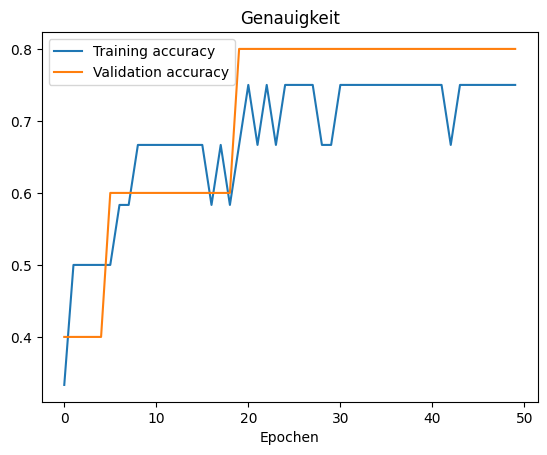
\includegraphics[width=.75\textwidth]{abbildungen/PlotAcc.png}
    \caption{Plot der Genauigkeit}
    \label{fig:plotAcc}
\end{figure}

\subsection{K-Cross-Validierung}
\label{chap:kCross}

Eine Möglichkeit zur besseren Beurteilung eines Modells wäre die k-cross-Validierung. Bei diesem Verfahren werden die Daten in k Teilmengen aufgeteilt
und k Modelle erstellt. Jedes Modell wird mit k-1 Teilmengen trainiert, die letzte Teilmenge wird zum Testen verwendet \cite[vgl. S.121f.]{DL_PY}. Abbildung \ref*{fig:kCross} zeigt
schematisch das Verfahren für k=3. Das endgültige Ergebnis ist definiert als der Durchschnitt der einzelnen Teilergebnisse der Modelle. 

\begin{figure}[H]
    \centering
    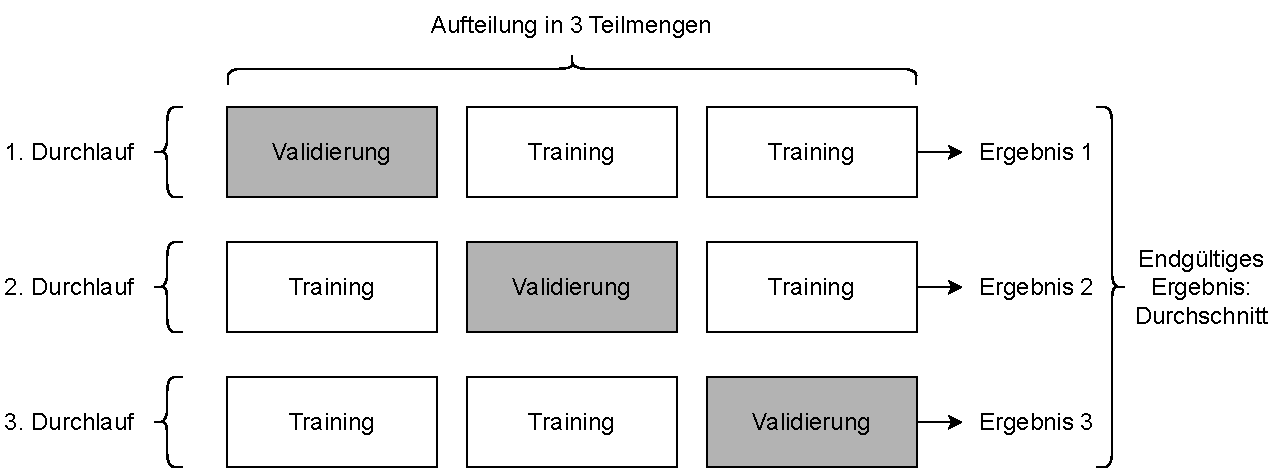
\includegraphics[width = \textwidth]{abbildungen/k_cross.pdf}
    \caption{k-cross-Validierung}
    \label{fig:kCross}
\end{figure}

Um eine k-cross-Validierung durchzuführen, müssen nacheinander Modelle erstellt werden, die mit verschiedenen Teilmengen des Datensatzes trainiert und getestet werden.
Die dafür benötigten Schritte werden im Quellcode \ref*{lst:kCross} gezeigt.
Dafür wird als Erstes definiert, wie viele Modelle und Teilmengen genutzt werden sollen, hier wird sich für vier entschieden. 
Danach wird eine Schleife viermal durchlaufen und bei jeder Iteration wird der Trainings- und Testdatensatz neu definiert. Der Testdatensatz besteht dabei 
aus 25~\% des Datensatzes, in der ersten Iteration aus den ersten 25~\%, bei der zweiten die nächsten 25~\% und so weiter. Der Trainingsdatensatz beinhaltet die restlichen
Daten. Innerhalb der Schleife werden danach die Daten wieder in Ein- und Ausgabewerte aufgeteilt, dieses Mal müssen auch die Testdaten entsprechend aufgeteilt werden.
Danach kann wieder das Modell definiert und angelernt werden. Da der Testdatensatz nun selber definiert wurde, kann nicht mehr auf die automatische Aufteilung zurückgegriffen werden.
Jetzt müssen die Testdaten, aufgeteilt in Ein- und Ausgabewerte, der Methode übergeben werden. Zudem wurde hier die Anzahl an Epochen auf 250 erhöht, damit beobachtet werden kann,
wie das Modell sich bei steigender Anzahl an Epochen verhält. Das zurückgegebene Objekt der fit()-Methode wird genutzt, um die vier verschiedene Werte jeweils in Listen speichern 
zu können, damit der Verlauf wieder visualisiert werden kann.
\begin{lstlisting}[language = python, caption={Aufteilung des Datensatzes in Teilmengen},captionpos=b, label = lst:kCross, float, floatplacement=H]
    num_epochs = 250
    k = 4
    for i in range(k):
        start = int(i/k * len(df_training))
        end = int((i/k + 0.25) * len(df_training))
        val_data = df_training.iloc[start:end] 
        train_data = df_training.drop(range(start,end))
        #...
        history = model.fit(trainX, trainYStatus,
                            batch_size=2,
                            epochs=num_epochs,
                            verbose=2,
                            validation_data=(valX, valYStatus))
        all_val_loss.append(history.history['val_loss'])
        all_loss.append(history.history['loss'])
        all_acc.append(history.history['categorical_accuracy'])
        all_val_acc.append(history.history['val_categorical_accuracy'])
\end{lstlisting}

Der Wert der Verlustfunktion sowie die Genauigkeit müssen noch gemittelt werden. Dafür wird, wie der Quellcode \ref*{lst:Durchschnitt} zeigt, der Durchschnitt 
der vier Kenngrößen pro Epoche gebildet. Mit den Werten können im nächsten Schritt wieder Diagramme zur Visualisierung erstellt werden.
\begin{lstlisting}[language = python, caption={Mitteln der Ergebnisse \cite{DL_PY}},captionpos=b, label = lst:Durchschnitt, floatplacement=H]
    avg_val_loss = [np.mean([x[i] for x in all_val_loss])
                    for i in range(num_epochs-1)]
    avg_loss     = [np.mean([x[i] for x in all_loss])
                        for i in range(num_epochs-1)]
    avg_acc      = [np.mean([x[i] for x in all_acc])
                        for i in range(num_epochs-1)]
    avg_val_acc  = [np.mean([x[i] for x in all_val_acc])
                        for i in range(num_epochs-1)]
\end{lstlisting}
Die Abbildungen \ref*{fig:kCrossLoss} und \ref*{fig:kCrossAcc} zeigen das Ergebnis der k-cross-Validierung. Bei der Verlustfunktion wird deutlich, dass
der Wert der Verlustfunktion auf den Testdaten bis ca. 80 Epochen leicht abnimmt, danach aber ansteigend, während der Wert der Verlustfunktion 
auf den Trainingsdaten abnimmt und gegen ca. 0,2 konvergiert. Das Ansteigen auf den Testdaten und Abnehmen auf den Trainingsdaten ist ein Zeichen dafür,
dass das Modell die Trainingsdaten auswendig lernt und die Generalisierungsfähigkeit des Modells darunter leidet und somit Overfitting auftritt.

Das Diagramm zur Genauigkeit zeigt, dass mehr Epochen nicht automatisch ein besseres Ergebnis liefern. Auf den Testdaten ändert sich die Genauigkeit 
ab der fünfzigsten Epoche nicht mehr wesentlich und stagniert ab Epoche 150. Im Vergleich zur Genauigkeit in der Abbildung \ref*{fig:plotAcc} 
ist der Durchschnitt der Genauigkeit von vier Modellen geringer. Daran kann erkannt werden, dass die Testdaten bei \ref*{fig:plotAcc} für das Modell günstig 
waren und das Modell auf diesen Daten gute Leistungen bringen konnte, was jedoch nicht so viel über die Leistung auf anderen Daten aussagt, da der Datensatz zu klein ist. 
Gerade in diesem Fall bietet sich die k-cross-Validierung sehr an und bietet wesentlich verlässlichere Kenngrößen als das Testen mit einem Modell auf einem 
Testdatensatz \cite[vgl. S.123]{DL_PY}.

\begin{figure}[H]
    \centering
    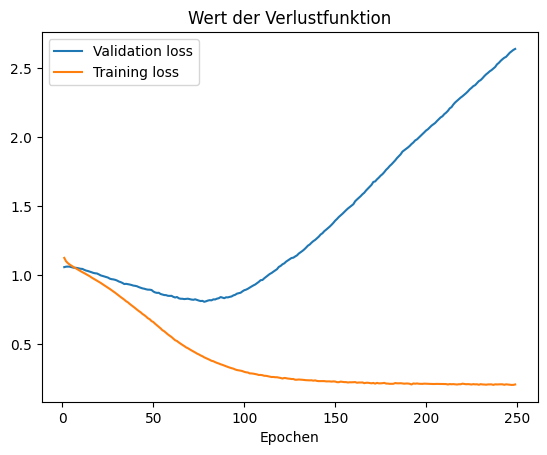
\includegraphics[width=.75\textwidth]{abbildungen/kCrossLoss.png}
    \caption{Verlustfunktion nach k-cross-Validierung}
    \label{fig:kCrossLoss}
\end{figure}
\begin{figure}[H]
    \centering
    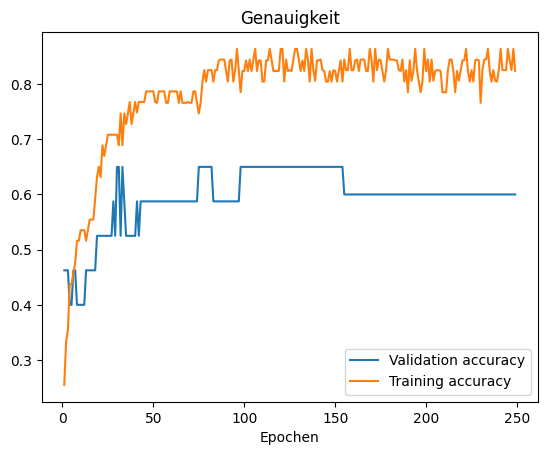
\includegraphics[width=.75\textwidth]{abbildungen/kCrossAcc.png}
    \caption{Genauigkeit nach k-cross-Validierung}
    \label{fig:kCrossAcc}
\end{figure}

\section{Verbesserungen des ersten Modells}
\label{chap:VerbesserungenNN}

In Kapitel \ref*{chap:DefineNN} wurde gezeigt, wie ein Modell für die Vorhersage für den Statuswert aussehen kann. Diese Schritte müssten ebenfalls für das dazugehörige Statement
durchlaufen werden. Das Ergebnis wären zwei unabhängige Modelle, die beide jeweils einzeln und nacheinander trainiert werden müssen. Diese Aufteilung ist nötig gewesen,
da die \glqq Sequential\grqq{}-Klasse es nicht erlaubt, mehrere Ausgabeschichten zu definieren und da die \glqq softmax\grqq{}-Funktion allen Ausgabeneuronen 
einen Wert zuordnet, die addiert eins ergeben. Um dieses Problem zu umgehen, kann statt der \glqq Sequential\grqq{}-Klasse von Keras, 
ein \ac{API}, die funktionale Keras-\ac{API}, verwendet werden. 
Dadurch wird es ermöglicht, Modelle zu definieren, die mehr als eine Eingabe- oder Ausgabeschicht haben oder Verzweigungen zwischen den Layern besitzen \cite[vgl. S.299f.]{DL_PY}. 
Abbildung \ref*{fig:FunktionaleAPI} zeigt den Aufbau eines \ac{NN} mit zwei Ausgabeschichten. Genau so ein Modell wird im nächsten Schritt mit der funktionalen Keras-\ac{API} erstellt.

\begin{figure}[H]
    \centering
    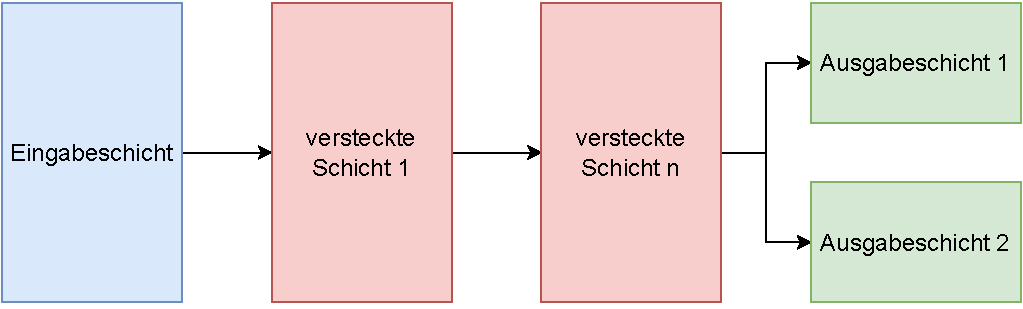
\includegraphics[width=\textwidth]{abbildungen/NN_funktionaleAPI.pdf}
    \caption{Modell mit zwei Ausgabeschichten}
    \label{fig:FunktionaleAPI}
\end{figure}

Grundsätzlich ist es möglich jedes Modell, welches mit der \glqq Sequential\grqq{}-Klasse erstellt wurde, in ein Modell mit der funktionalen Keras-\ac{API} zu übersetzen. 
Deshalb wird als Erstes das bestehende und in Kapitel \ref*{chap:DefineNN} beschriebene Modell übersetzt und im Anschluss daran wird dem Modell eine zweite Ausgabeschicht
hinzugefügt.
Mit der funktionalen \ac{API} werden Tensoren direkt bearbeitet und können den Schichten, wie bei einer Funktion, übergeben und entgegengenommen werden. Ein Tensor ist eine
Datenstruktur, welche als n-dimensionales-Array beschrieben werden kann. Skalare sind Tensoren der Stufe 0, Vektoren sind Tensoren der Stufe 1, Matrizen sind Tensoren
der Stufe 2 und so weiter \cite[vgl. S.128]{AI_Huawei}. Ziel dabei ist es, 
aus einem Eingabetensor einen Ausgabetensor zu erzeugen. Dafür ruft die Bibliothek alle Schichten ab, die an dieser Transformation beteiligt sind, und fasst diese Struktur
anschließend als Modell zusammen. Der Ausgabetensor entsteht also durch aufeinanderfolgende Transformationen des Eingabetensors \cite[vgl. S.305]{DL_PY}. 
Quellcode \ref*{lst:SeqToFunc} zeigt die Definition des Modells aus Kapitel \ref*{chap:DefineNN} mit der funktionalen \ac{API} und kann mit Quellcode \ref*{lst:ModellSeq}
verglichen werden. 

\begin{lstlisting}[language = python, caption={Modell mit funktionaler \acs{API} darstellen},captionpos=b, label = lst:SeqToFunc, floatplacement=H]
    input = Input(shape=(trainX.shape[1],))
    x = Dense(8, activation='relu')(input)
    x = Dense(16, activation='relu')(x)
    output = Dense(trainYStatus.shape[1], activation='softmax')(x)
    model = Model(input, output)
    model.summary()
    ---------------------------------------
    Output:
    ______________________________________________________________
    Layer (type)                Output Shape              Param #   
    ==============================================================
    input_9 (InputLayer)        [(None, 177)]             0         
                                                                    
    dense_36 (Dense)            (None, 8)                 1424      
                                                                    
    dense_37 (Dense)            (None, 16)                144       
                                                                    
    dense_38 (Dense)            (None, 3)                 51        
                                                                    
    ==============================================================
    Total params: 1,619
    Trainable params: 1,619
    Non-trainable params: 0
    ______________________________________________________________

\end{lstlisting}

Anders als bei der Erstellung des Modells mit der \glqq Sequential\grqq{}-Klasse, wird hier die Dimension der Eingabedaten nicht in der ersten Schicht als Parameter übergeben,
sondern wird noch vorher festgelegt. Wie in der Zusammenfassung des Modells zu sehen ist, stellt \glqq Input\grqq{} jedoch keine wirkliche erste Schicht dar,
da sie keine Parameter besitzt. Bis auf diesen Unterschied ist die Zusammenfassung beider Modelle gleich. Der Prozess des Trainierens und die Auswahl der Verlustfunktion
sowie des Optimierers sind ebenfalls identisch. Deshalb sind beide Modelle in der Anwendung äquivalent. Nun muss noch eine weitere zusätzliche Ausgabeschicht hinzugefügt werden,
welche das Statement zur Bewertung der Anwendungsregel prognostizieren soll. Dafür werden Zeile vier und fünf des Quellcodes \ref*{lst:SeqToFunc} überarbeitet, was 
in Quellcode \ref*{lst:Outputs} gezeigt wird.
\\
\begin{lstlisting}[language = python, caption={Zweite Ausgabeschicht hinzufügen},captionpos=b, label = lst:Outputs, floatplacement=H]
   output1 = Dense(trainYStatus.shape[1], activation='softmax', 
       name='status')(x)
   output2 = Dense(trainYStatement.shape[1], activation='softmax', 
       name='statement')(x)
   model = Model(inputs=input, outputs=[output1, output2])
\end{lstlisting}

Beide Ausgabeschichten erhalten als Parameter die Anzahl an möglichen Ausprägungen ihres Zielattributs sowie eine Aktivierungsfunktion. An dieser Stelle wäre es auch
möglich verschiedene Aktivierungsfunktionen auszuwählen. Sollte beispielsweise ein Zielattribut das Ergebnis einer Regression sein, könnte hier auch 
\glqq mse\grqq{} gewählt werden. Zudem erhalten die beiden Layer noch einen eindeutigen Namen. Beim Aufruf der compile()-Methode besteht dadurch die Möglichkeit,
den beiden Schichten unterschiedliche Verlustfunktionen zuzuweisen \cite[vgl. S.308f.]{DL_PY}. Da beide Layer hier jedoch eine Single-Label-Mehrfachklassifizierung lösen sollen,
wird das nicht benötigt. 

Das Übersetzen der beiden Modelle mit der \glqq Sequential\grqq{}-Klasse in ein Modell mit der funktionalen \ac{API} hat den Vorteil, dass nun nur noch ein Modell 
erstellt und trainiert werden muss, was die Laufzeit des Modells halbiert und zudem Zeilen an Code spart.

\subsection{Wahl des Optimierers}

Wie in Kapitel \ref*{chap:DefineNN} beschrieben, ist es schwierig vorher zu bestimmen, welcher Optimierer die beste Performance liefert. Die Herangehensweise
um den idealen Optimierer zu finden ist daher Trial-and-Error. Dafür wird mit einer k-cross-Validierung der mittlere Wert der Verlustfunktion für den Statuswert
über mehrere Epochen und mit verschiedenen Optimierern visualisiert und anschließend geprüft, welcher Optimierer den niedrigsten Wert liefert. Es werden die Optimierer 
\glqq Adam\grqq{}, \glqq RMSprop\grqq{} und \glqq SGD\grqq{} ausprobiert.
Hier wird nur der Statuswert betrachtet, da das Statement bei den meisten Anwendungsregeln einzigartig ist und somit selten eine genaue Übereinstimmung vorhanden ist.
Deshalb ist beim Statement die Genauigkeit in der Regel null und darum ist der Wert der Verlustfunktion für das Statement nicht aussagekräftig.

\begin{figure}[H]
    \centering
    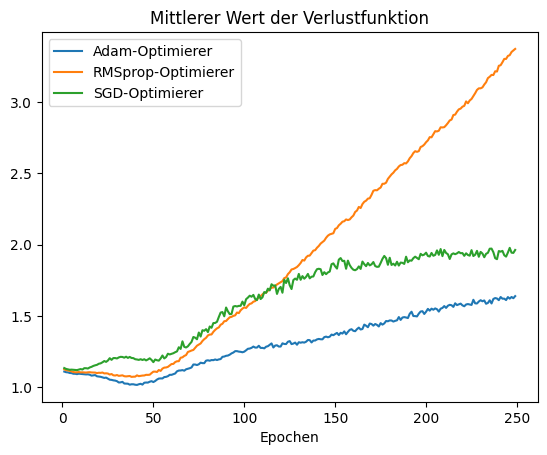
\includegraphics[width=.75\textwidth]{abbildungen/Optimierer/LossOptimierer.png}
    \caption{Vergleich verschiedener Optimierer}
    \label{fig:LossOptimierer}
\end{figure}

Das Diagramm in der Abbildung \ref*{fig:LossOptimierer} zeigt den Verlauf des mittleren Werts der Verlustfunktion über mehrere Epochen. Dort ist zu erkennen, dass 
der Adam-Optimierer insgesamt den niedrigsten Wert erreicht, weshalb dieser im Folgenden genutzt wird. Jedoch
unterscheiden sich die Werte mit den verschiedenen Optimierern bis zur ca. Epoche 50 nicht stark, weshalb davon auszugehen ist, dass die Wahl des Optimierers in diesem spezifischen
Anwendungsfall keine allzu große Rolle spielt.

Neben der Auswahl des Optimierers kann ebenfalls die Lernrate eine Rolle spielen. Die Lernrate ist ein Parameter, der den Optimierer beeinflusst, weshalb verschiedene Lernraten ausprobiert werden
sollten. Standardmäßig beträgt die Lernrate des Adam-Optimierers 0,001 \cite{KerasDoc}. Als weitere Lernraten werden 0,01 und 0,0001 gewählt, um zu prüfen, wie 
sich der Wert der Verlustfunktion ändert, wenn eine größere bzw. kleinere Lernrate gewählt wird.
Die Lernrate des Optimierers kann bei Aufruf der compile()-Methode festgelegt werden, wie der Quellcode \ref*{lst:Learnrate} zeigt.

\begin{lstlisting}[language = python, caption={Wahl der Lernrate},captionpos=b, label = lst:Learnrate, floatplacement=H]
    model.compile(optimizer=optimizers.Adam(learning_rate=0.0001),
        loss   ={'status': CategoricalCrossentropy(), 
                 'statement': CategoricalCrossentropy()},
        metrics=['categorical_accuracy'])
\end{lstlisting}

Abbildung \ref*{fig:LossLR} zeigt den Verlauf der Verlustfunktion mit den drei verschiedenen Lernraten. Deutlich zu erkennen ist, dass ein Vergrößern der Lernrate zu 
einem wesentlich schlechteren Ergebnis führt. Die standardmäßige sowie die kleinere Lernrate ähneln sich in ihrem Verlauf, wobei die standardmäßige Lernrate
ein tieferes Minimum erreicht, weshalb der Wert der Lernrate in diesem Fall nicht verändert werden sollte.

\begin{figure}[H]
    \centering
    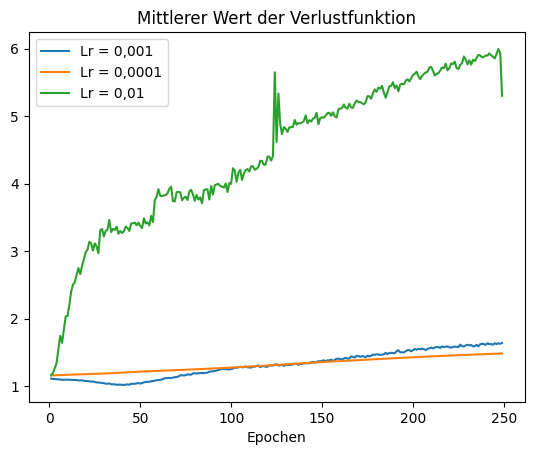
\includegraphics[width=.75\textwidth]{abbildungen/Optimierer/LossLR.png}
    \caption{Vergleich verschiedener Lernraten}
    \label{fig:LossLR}
\end{figure}

\subsection{Anpassen der Modellarchitektur}
Nachdem mehrere Optimierer ausprobiert und sich für einen entschieden wurde, sollte im nächsten Schritt noch geprüft werden, ob durch eine Anpassung der Modellarchitektur
gegebenenfalls ein besseres Ergebnis erzielt werden kann. Ähnlich wie bei der Wahl des Optimierers im vorherigen Schritt, wird dies wieder durch Ausprobieren und 
anschließendes Visualisieren entschieden. Dabei wird die Anzahl an Schichten sowie die Anzahl an Neuronen in einer Schicht angepasst.
Zudem wird geprüft, ob mittels einer Dropout-Regularisierung ein besseres Ergebnis erzielt werden kann. 
Folgende Modellarchitekturen werden dargestellt:
\\
\begin{description}[style=multiline,leftmargin=3cm,font=\bfseries, nolistsep]
    \item[M1] Modell mit zwei versteckten Schichten (32, 16 Neuronen)
    \item[M2] breiteres und tieferes Modell mit vier Schichten (256, 128, 64, 32 Neuronen) mit Dropout-Regularisierung
    \item[M3] breiteres und tieferes Modell mit vier Schichten (256, 128, 64, 32 Neuronen) ohne Dropout-Regularisierung
    \item[M4] Modell mit einer versteckten Schicht mit 16 Neuronen
    \item[M5] Modell mit einer versteckten Schicht mit 512 Neuronen
\end{description}
Ein Beispiel für eine Dropout-Regularisierung zeigt der Quellcode \ref*{lst:Dropout}. Die Dropout-Klasse erwartet als Parameter einen Wert zwischen null und eins. 
Dieser Wert stellt den Anteil an Neuronen dar, dessen Ausgabe während des Trainings auf null gesetzt wird.
\begin{lstlisting}[language = python, caption={Dropout-Regularisierung mit Keras},captionpos=b, label = lst:Dropout, floatplacement=H]
    x = Dense(256, activation='relu')(inputs)
    x = Dropout(0.2)(x)
    x = Dense(128, activation='relu')(x)
\end{lstlisting}
Der Verlauf des mittleren Wertes der Verlustfunktion wird in Abbildung \ref*{fig:LossModelle} für alle fünf Modelle dargestellt. Zu erkennen ist, dass die beiden Modelle mit 
der geringsten Anzahl an Neuronen (M1 und M4) die besten Ergebnisse erzielen, während die beiden Modelle mit der höchsten Komplexität (M2 und M3) die schlechtesten Ergebnisse
erzielen. Der Grund dafür ist vermutlich, dass die komplexeren Modelle zu komplex sind um das Problem zu lösen. Zudem wird der kleine Datensatz ebenfalls dafür sorgen,
dass simplere Modelle in diesem Anwendungsfall bessere Leistungen erzielen. Auch die Dropout-Regularisierung bringt in diesem Anwendungsfall kein besseres Ergebnis. Das Minimum
des Modells M1 lässt sich mit der argmin()-Methode der Numpy-Bibliothek bestimmen. Bei Epoche 23 hat M1 sein globales Minimum. Deshalb sollte dieses Modell weiterhin genutzt werden
und beim Trainieren des Modells sollte als Anzahl an Epochen ein Wert um 23 gewählt werden, um ein bestmögliches Ergebnis in diesem Anwendungsfall zu erreichen.

\begin{figure}[H]
    \centering
    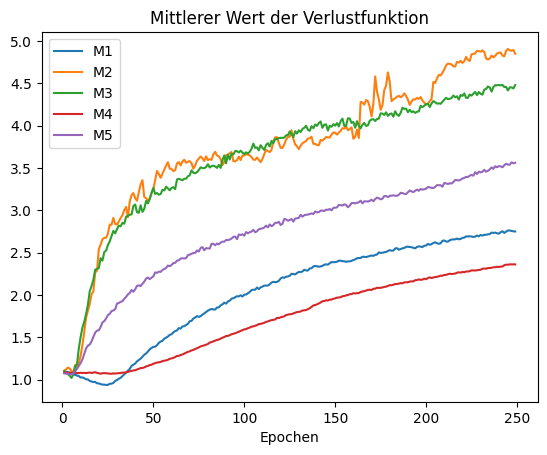
\includegraphics[width=.75\textwidth]{abbildungen/LossModelle.png}
    \caption{Vergleich verschiedener Modellarchitekturen}
    \label{fig:LossModelle}
\end{figure}

\section{Vorhersagen treffen}
\label{chap:Prediction}

Da nun ein Modell definiert und mit Daten angelernt wurde, sollen mögliche Vorhersagen zur Bewertung von Anwendungsregeln getroffen werden. 
Um die Anwendung des Modells vorzustellen, wurde vor dem Trainingsprozess eine Zeile aus dem Trainingsdatensatz entfernt. 
Das Modell soll nun zu dieser Zeile einen Vorschlag zur Bewertung abgeben. Zum Treffen von Vorhersagen kann 
die Methode predict() der Keras-Bibliothek benutzt werden. Mit dieser Methode können einem trainierten Modell neue Daten übergeben werden.
Anhand dieser Daten erstellt das Modell dann eine Vorhersage. Quellcode \ref*{lst:Predict} zeigt, wie so eine Vorhersage getroffen werden kann.
Da das Modell zwei Ausgabeschichten besitzt, gibt diese Methode auch zwei Objekte zurück. Diese Objekte sind Listen, welche die Wahrscheinlichkeiten
der einzelnen Ausprägungen beinhalten. Über diese Liste kann iteriert werden, um diese Wahrscheinlichkeiten auszugeben. Für den Statuswert 
wurden alle möglichen Ausprägungen ausgegeben, da dort nur drei Verschiedene vorhanden sind. Aufgrund der Übersichtlichkeit wird für das Statement
nur der Text ausgegeben, der die höchste Wahrscheinlichkeit besitzt. 
\begin{lstlisting}[language = python, caption={Vorhersage über neue Daten treffen},captionpos=b, label = lst:Predict, floatplacement=H]
    prediction_status, prediction_statement = model.predict(test)

    for val in prediction_status:
        for col in range(len(val)):
            print (str(trainYStatus.columns[col]) + " " + 
                   '{:.1%}'.format(val[col]))
    
    index_max = np.argmax(prediction_statement)
    for val in prediction_statement:
        print (trainYStatement.columns[index_max] + " " + 
               '{:.1%}'.format(val[index_max]))
\end{lstlisting}
Der tatsächliche Statuswert des Beispiels ist \glqq compliant\grqq{}. Die Ausgabe für den vorhergesagten Statuswert sieht wie folgt aus:
\begin{quotation}
    \noindent closed 2.0~\%\\
    compliant 88.2~\%\\
    not applicable 9.8~\%
\end{quotation}
Vergleicht man diese Ausgabe mit der Verteilung der Statuswerte der beispielhaft bewerteten Anwendungsregel in Abbildung \ref*{fig:StatusTest}, erkannt man eindeutig, 
dass das Modell eine Struktur erkennt und in der Lage ist, den Statuswert einer Anwendungsregel vorherzusagen.
\begin{figure}[H]
    \centering
    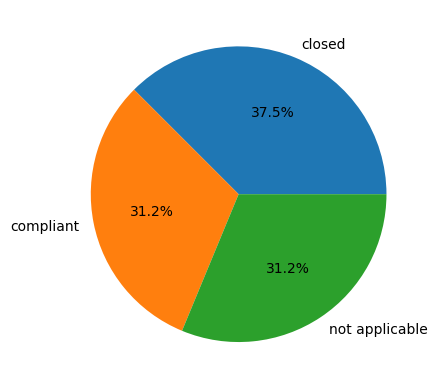
\includegraphics[width=.5\textwidth]{abbildungen/StatusTest.png}
    \caption{Verteilung des Statuswerts der betrachteten Anwendungsregel}
    \label{fig:StatusTest}
\end{figure}
\pagebreak
Das tatsächliche dazugehörige Statement lautet: 
\begin{quotation}
    \noindent Im Projekt ... sind die Signalkabel nach VDE0816/2 verwendet. Die Verlegevorschriften des Kabels sind beim Verlegen eingehalten. Daher ist diese Auflage erfüllt.  
    Bitte sieh  Kabelspezifikation (Aussenkabel)  A6Z00038004325  -  Outdoor Cable Plan  A6Z00037954383  -
\end{quotation}
Folgendes wurde vom Modell prognostiziert:
\begin{quotation}
    \noindent Zur Anschaltung der Weichen in der Außenanlage kommen Signalkabel nach  VDE 0816/2 oder Kabel mit vergleichbaren Eigenschaften zum Einsatz. Siehe  auch Dokument Requirement for 
    Signalling cable G68167-S0100-U-5009   A6Z08110839230  01.  20.8~\%
\end{quotation}
Wie bereits erwähnt, sind die meisten Statements einzigartig. Hier wurde jedoch ein Statement gewählt, welches vom Inhalt her identisch ist. Anhand der beiden vorhergesagten Attribute
kann geschlussfolgert werden, dass das Modell in der Lage ist eine Struktur beim Bewerten von Anwendungsregeln zu erkennen und Ähnlichkeiten in den Projekten festzustellen. Das war jedoch
nur ein Beispiel für eine bewertete Anwendungsregel. Im Anschluss gilt es noch, dieses Modell zu testen, im Idealfall mithilfe eines größeren Datensatzes.



% ***************************** BIBLIOGRAPHY **********************************
\baselineskip=14pt
\clearpage
\phantomsection
\addcontentsline{toc}{chapter}{\protect\numberline{}\bibname}
\bibliography{bib/thesis}

% ******************************* APPENDIX ************************************
%\appendix
%\chapter{Anhang A}
\label{chap:anhang_a}

\begin{figure}[ht]
    \centering
    \begin{minipage}[t]{0.45\linewidth}
        \centering
        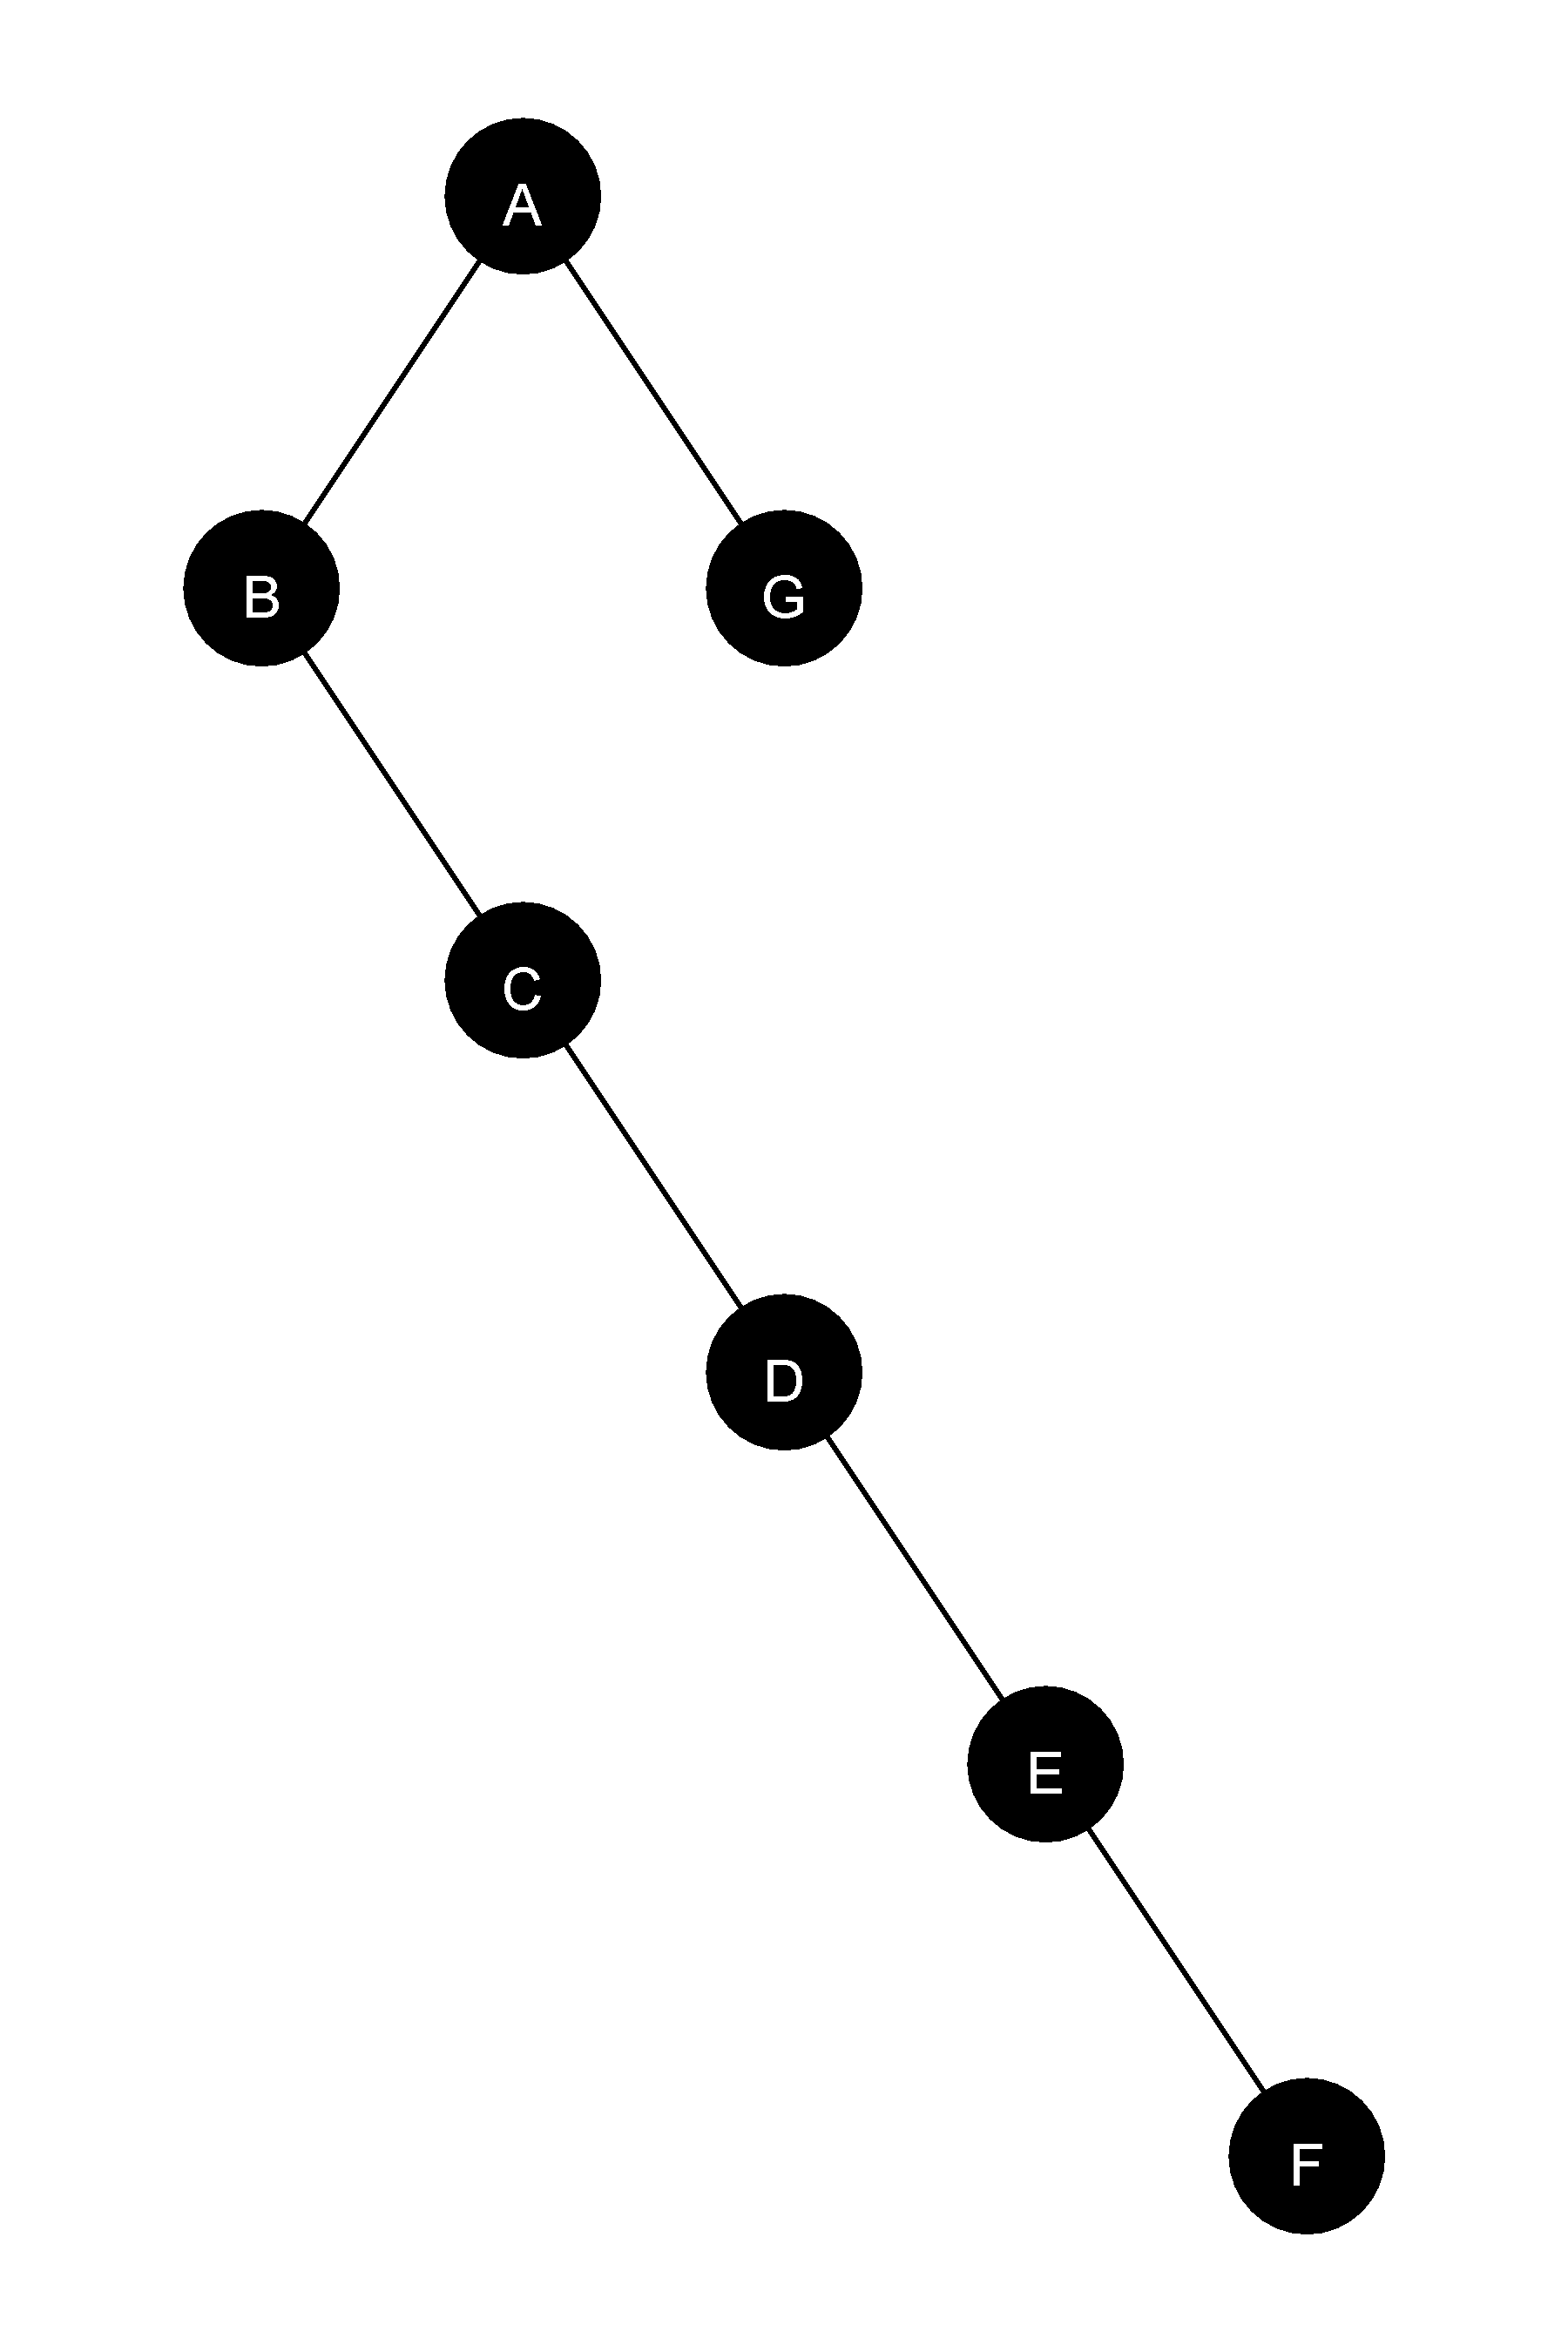
\includegraphics[scale = 0.06]{abbildungen/tree_spiegel_1_a2}
    \end{minipage}
    \hfill
    \begin{minipage}[t]{0.45\linewidth}
        \centering
        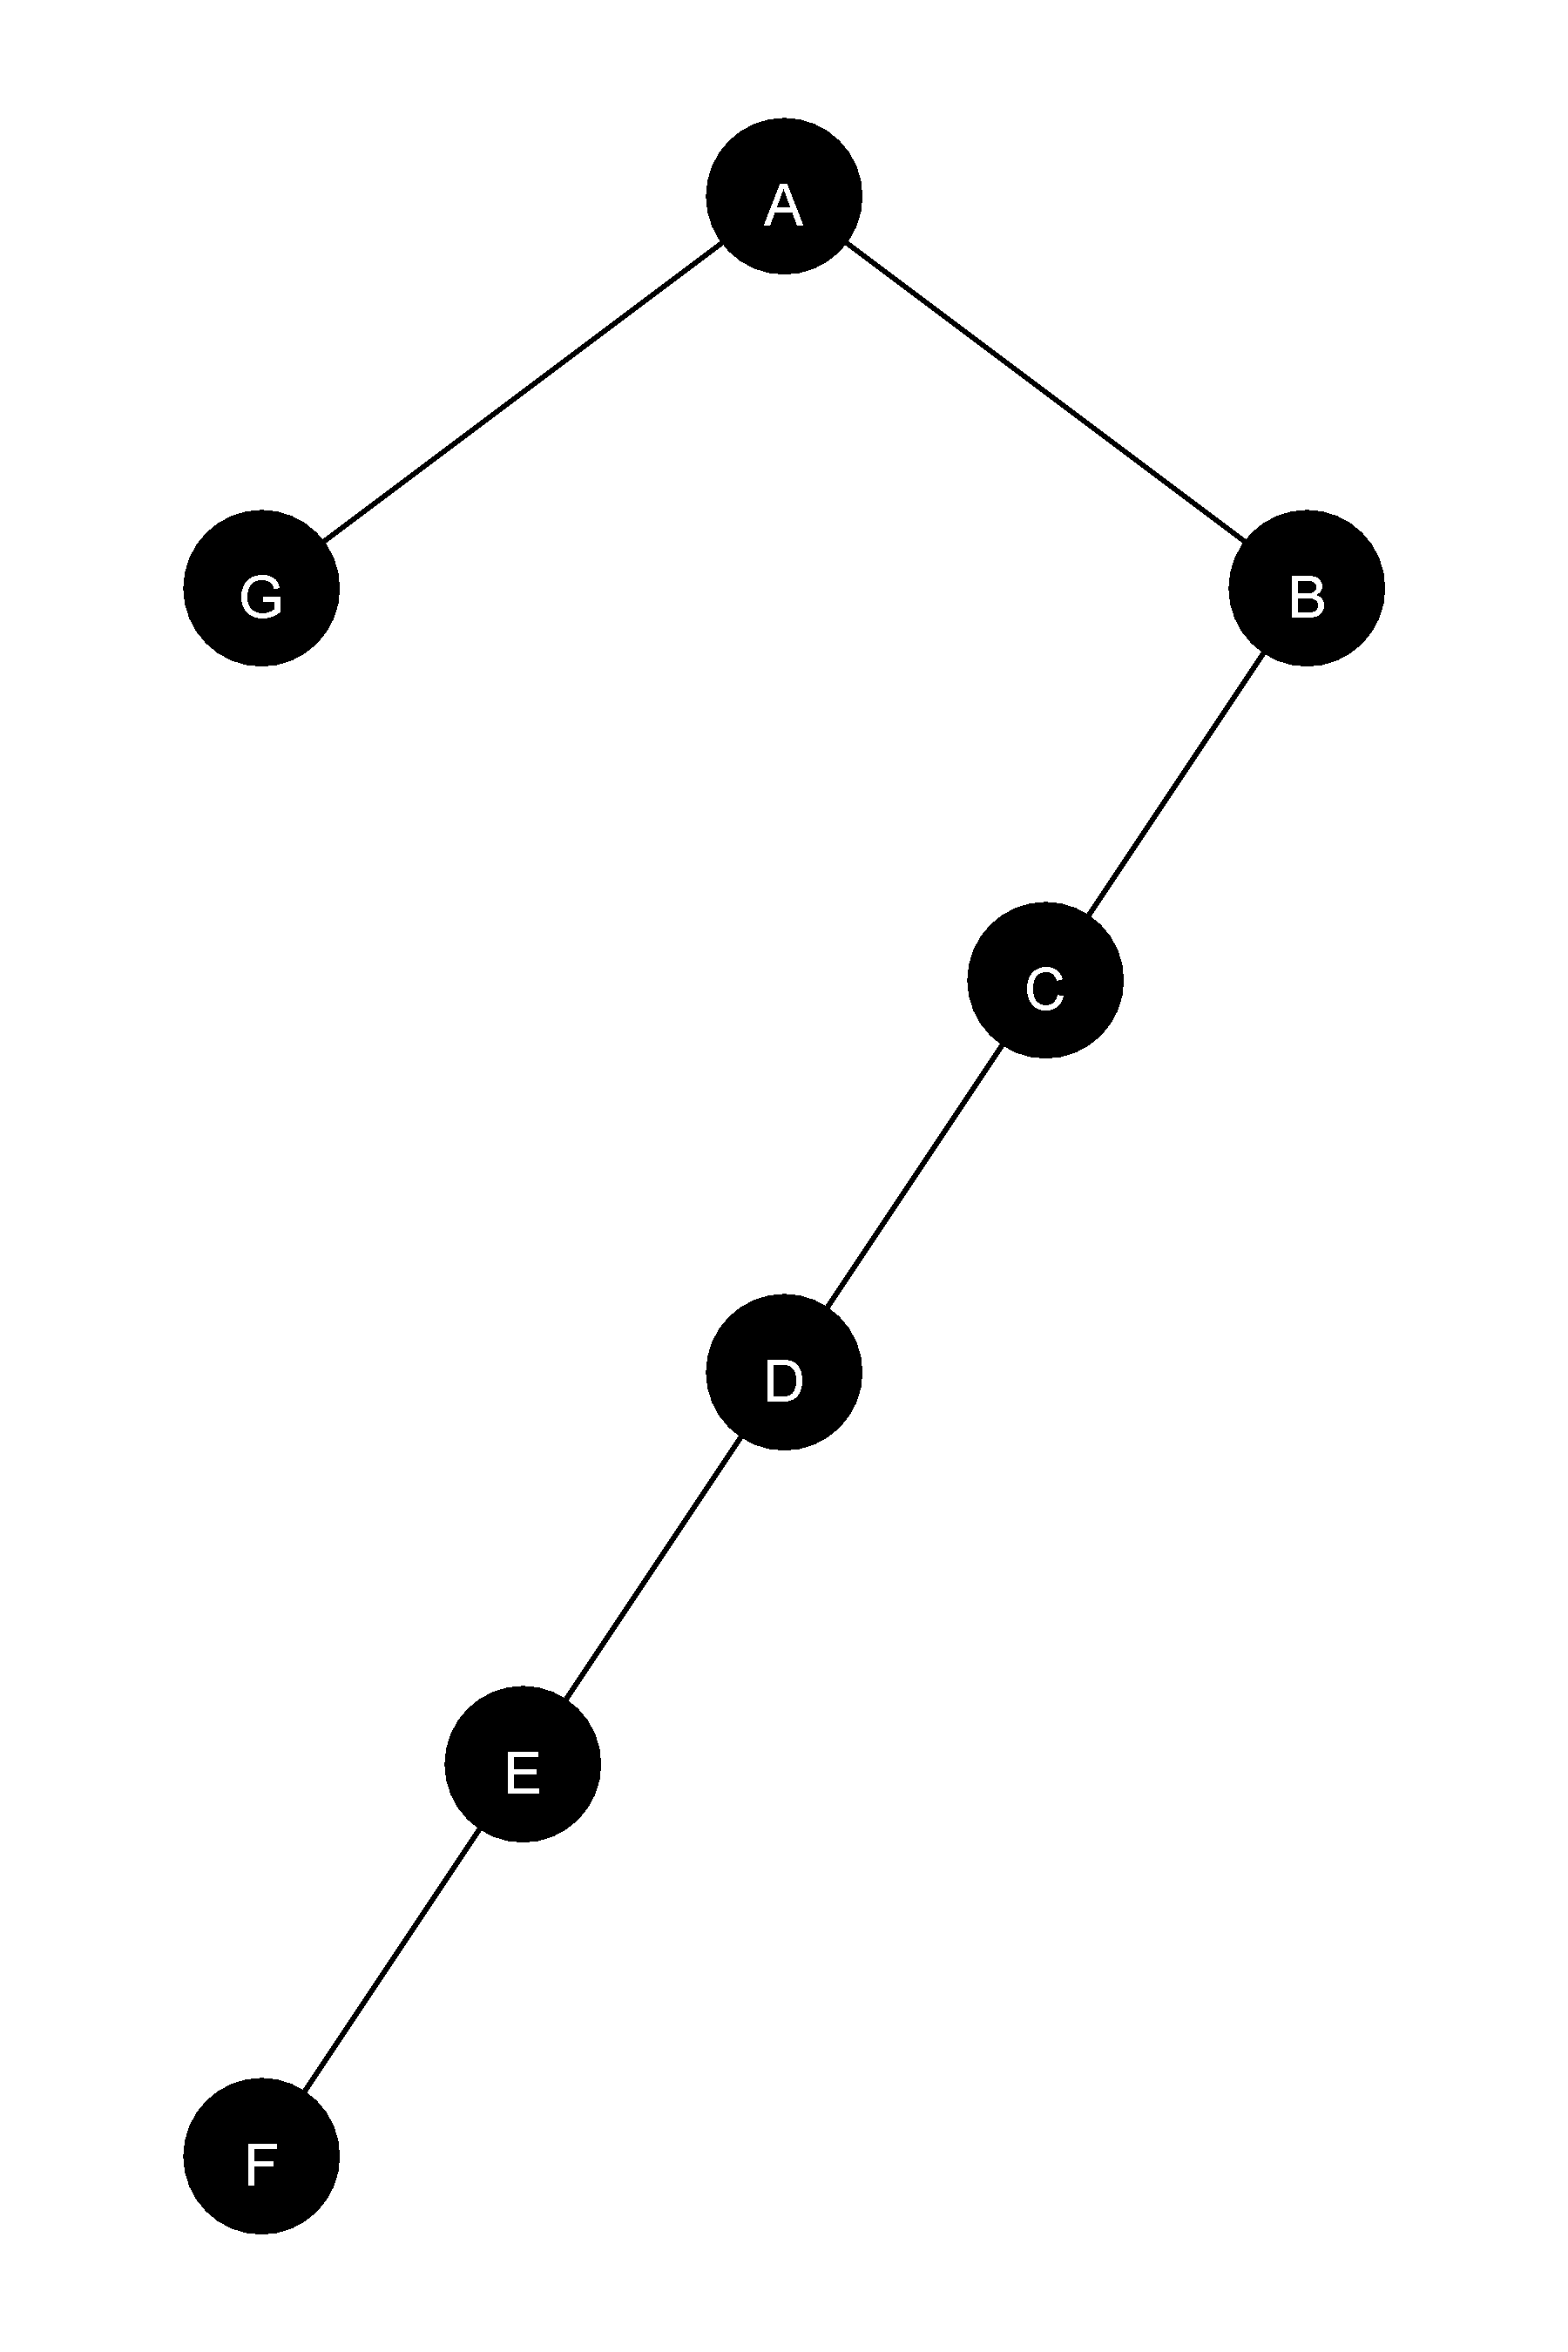
\includegraphics[scale = 0.06]{abbildungen/tree_spiegel_2_a2}
    \end{minipage} 
    \caption[]{Baum und Spiegelung gezeichnet nach WS}
    \label{pic:WS_Spiegel}
\end{figure}

\begin{figure}[ht]
    \centering
    \begin{minipage}[t]{0.45\linewidth}
        \centering
        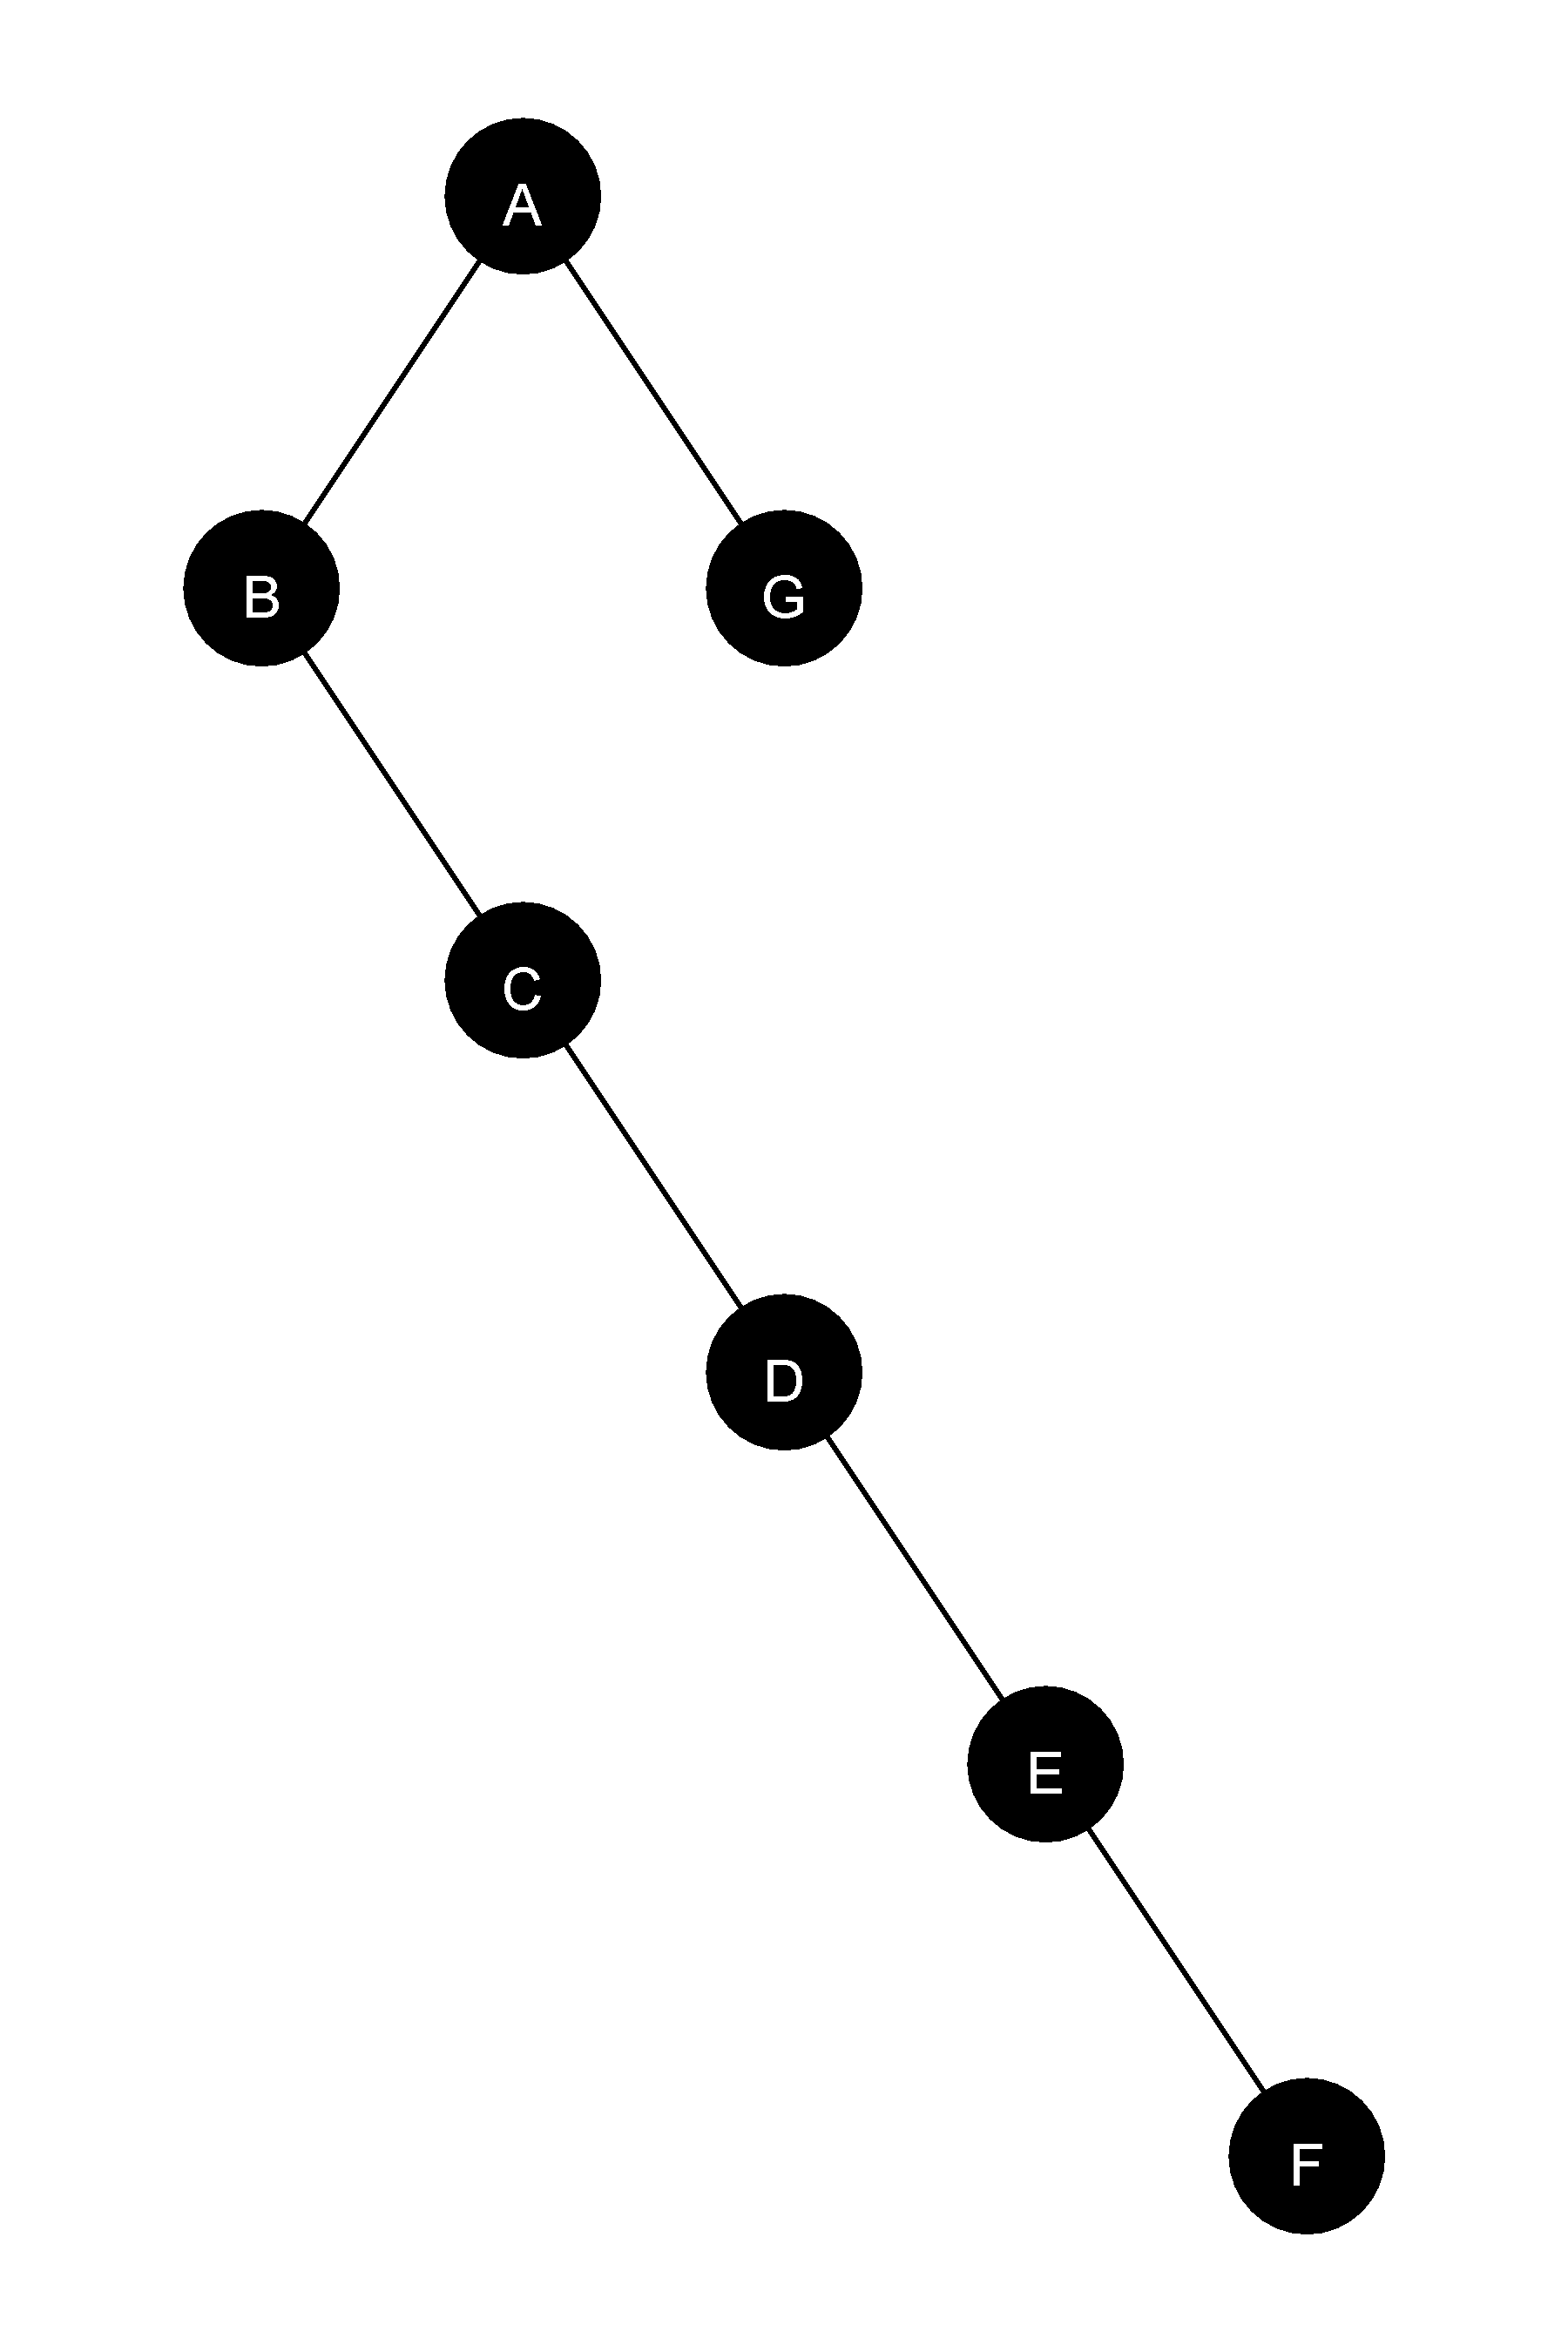
\includegraphics[scale = 0.06]{abbildungen/tree_spiegel_1_a3}
    \end{minipage}
    \hfill
    \begin{minipage}[t]{0.45\linewidth}
        \centering
        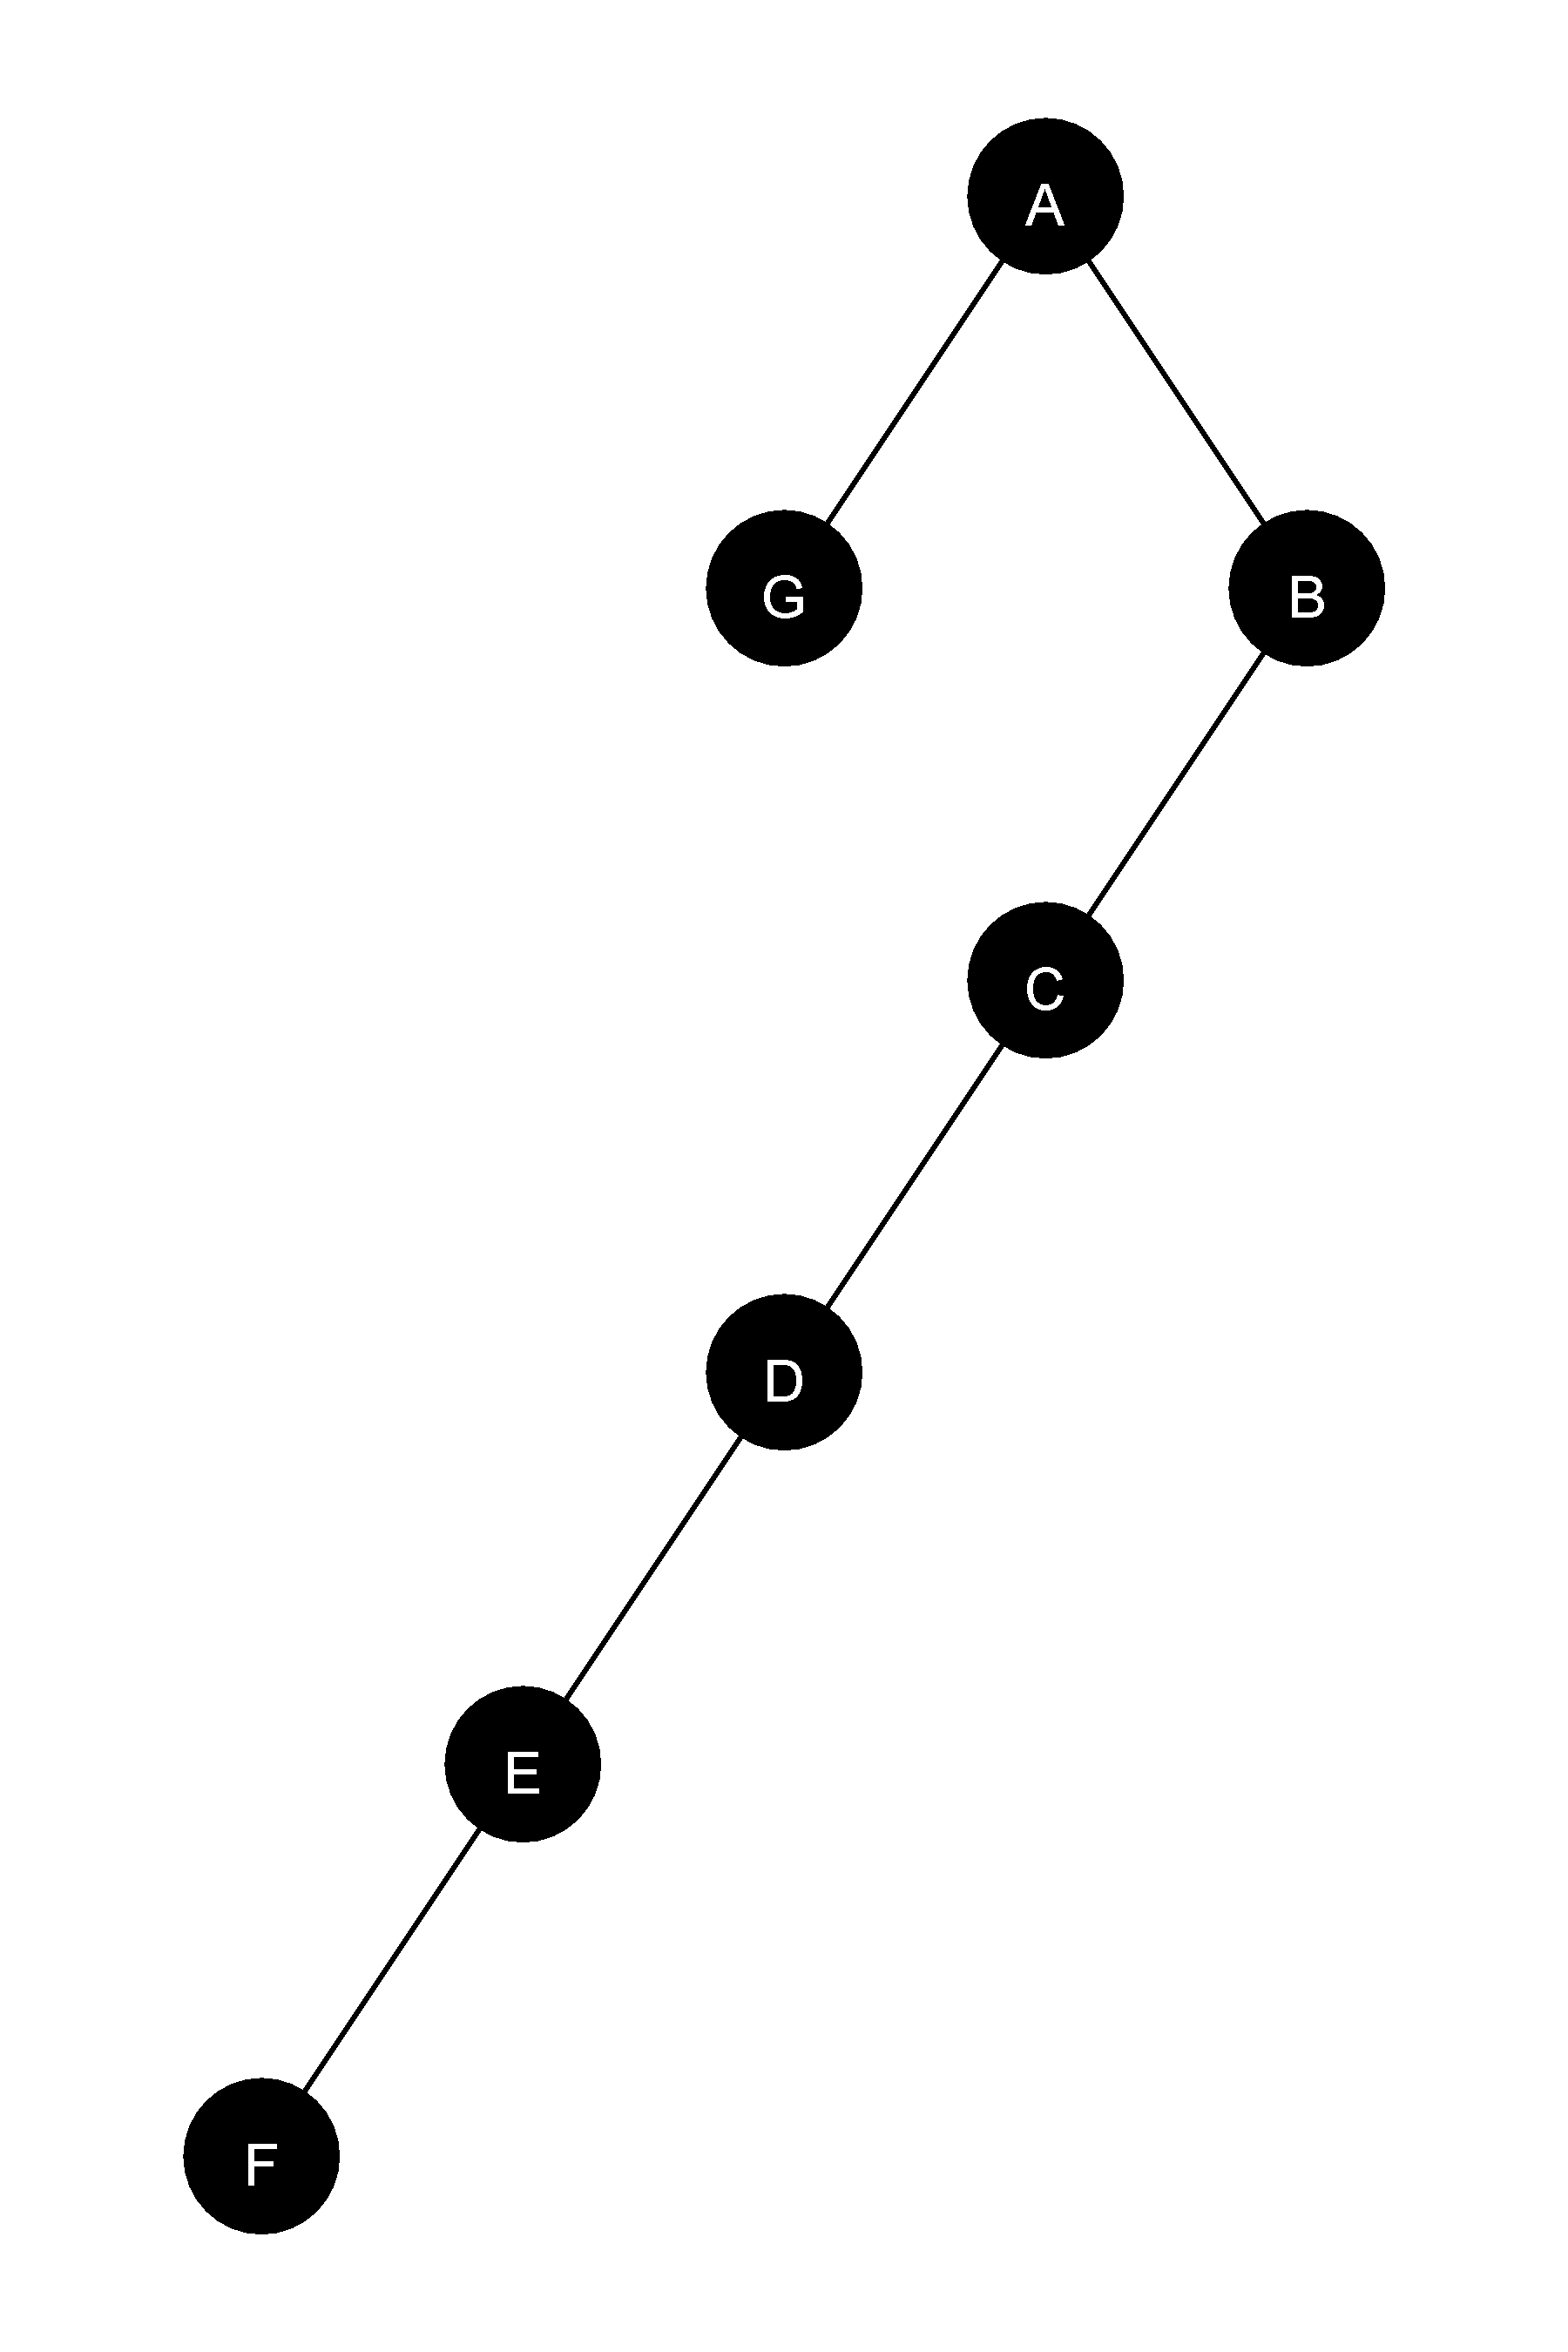
\includegraphics[scale = 0.06]{abbildungen/tree_spiegel_2_a3}   
    \end{minipage}  
    \caption[]{Baum und Spiegelung gezeichnet nach TR}
    \label{pic:TR_Spiegel}
\end{figure}

\chapter{Anhang B}
\label{chap:anhang_b}

\lstinputlisting[caption={Knoten-Klasse}]{abbildungen/git/src/algos/Knoten.java}

\lstinputlisting[caption={Binary-Klasse}]{abbildungen/git/src/algos/BinaryKnoten.java}

\lstinputlisting[caption={WS-Naiver-Algorithmus-Klasse}]{abbildungen/git/src/algos/NaiverAlgorithmus.java}

\lstinputlisting[caption={WS-Algorithmus-Klasse}]{abbildungen/git/src/algos/VerbesserterAlgorithmus.java}

\lstinputlisting[caption={RT-Algorithmus-Klasse}]{abbildungen/git/src/algos/TilfordAlgorithmus.java}

\lstinputlisting[caption={Zusatzklasse: Trees}]{abbildungen/git/src/algos/Trees.java}

\lstinputlisting[caption={Zusatzklasse: Drawer}]{abbildungen/git/src/algos/Drawer.java}

\lstinputlisting[caption={Zusatzklasse: Mains}]{abbildungen/git/src/algos/Mains.java}

% ***************************** BACK MATTER ***********************************
%\thispagestyle{empty}

%\addcontentsline{toc}{chapter}{\protect\numberline{}Eidesstattliche Erklärung}
%\chapter*{}
\vspace*{0.5cm}
\noindent

Hiermit versicheren wir, dass wir die vorliegende Arbeit selbstständig verfasst und keine anderen als die angegebenen Quellen und Hilfsmittel benutzt haben. Wir versicheren, dass wir alle wörtlich oder sinngemäß aus anderen Werken übernommenen Aussagen als solche gekennzeichnet haben, und dass die eingereichte Arbeit weder vollständig noch in wesentlichen Teilen Gegenstand eines anderen Prüfungsverfahrens gewesen ist.

\vspace{3cm}
\toponym, den \today

\end{document}